\documentclass{article}
\usepackage{verbatim}
\usepackage{amsmath}
%\usepackage[margin=1in,left=1.5in,includefoot]{geometry}
\usepackage{graphicx}
\usepackage{systeme}
\usepackage{listings}
\usepackage{color}
\usepackage{xcolor}
\usepackage{graphicx}
\usepackage{biblatex}
\usepackage{float}
\usepackage{hyperref}
\usepackage{placeins}
\usepackage{fancyhdr}
\usepackage[margin=1in]{geometry}

\usepackage{caption}
\captionsetup{font=footnotesize}


\definecolor{mygreen}{RGB}{28,172,0} % color values Red, Green, Blue
\definecolor{mylilas}{RGB}{170,55,241}
\pagestyle{fancy}
\fancyhead{}
\fancyfoot{}
\fancyfoot[R]{ \thepage\ }
\usepackage[utf8]{inputenc}

% Default fixed font does not support bold face
\DeclareFixedFont{\ttb}{T1}{txtt}{bx}{n}{12} % for bold
\DeclareFixedFont{\ttm}{T1}{txtt}{m}{n}{12}  % for normal

% Custom colors
\usepackage{color}
\definecolor{deepblue}{rgb}{0,0,0.5}
\definecolor{deepred}{rgb}{0.6,0,0}
\definecolor{deepgreen}{rgb}{0,0.5,0}

\addbibresource{Reference3.bib}



\begin{document}


\begin{titlepage}
  \begin{center}

    \huge
    \textbf{Final Report}\\
   % \vfill
    \vspace{4.5cm}
    \LARGE
    Group 2: Yujin Liu, Helen Jin, Jiangmeng Li\\
    \vspace{4.5cm}
    \Large
    CAAM37830\\
    \vspace{1cm}
    University of Chicago\\
    \vspace{1cm}
    December 8, 2020

  \end{center}

\end{titlepage}

\section{Abstract}
In this report, we investigated how the infectious disease spread throughout the population based on the susceptible-infected-recovered (SIR) epidemic model. We first ran the simulation with both the discrete agent-based and the continuous ODE models. We then proposed and implemented three variations of the model. In the first modification, we aim to understand how the usage of mask will change the way infectious disease spread, and how the adoption of the masks with different effectiveness influences rate of hospitalization and deaths. Secondly, we used some default parameters to fit the Covid-19 data from Hubei, China with continuous SIR model. Finally, we created the interactive time series plots of the daily confirmed cases and deaths for states, and the interactive US map of cumulative confirmed cases. Apart from these variations, we also added the a 2-dimensional spatial component to both the discrete agent-based and the continuous ODE models where population is confined in a grid and observe how different initial location conditions change the spread of the disease.

\section{Introduction}
The susceptible-infected-recovered (SIR) model is one of the compartmental models that simplify the mathematical modeling to the spread of infectious disease, where the time dependent variables $S$, $I$, $R$ each represent the following populations:

$S$(susceptible): number of individuals who are not infected but could become infected

$I$(infected): number of individuals who are already infected and can spread disease

$R$(recoverd): number of individuals who are either recovered and immune or have died

Additionally, $s$, $i$, $r$ are used to represent the proportion of susceptible, infected and recovered individuals among the population. This model assumes the susceptible population $S$ decreases monotonically towards 0, and the population size is fixed, and the duration of infectivity is same as length of the disease. There are two parameters $b$ and $k$ in the model, where $b$ indicates the number of interactions each day that could spread the disease (per individual) and $k$ indicates the fraction of the infectious population which recovers each day.

Generally, there are two kinds of SIR model, ODE and agent based model. The ODE model consists of the following system of the nonlinear ordinary differential equations, where $t$ is time:

$$\frac{ds}{dt} = -b * s(t) * i(t), \hspace{0.1cm}
\frac{dr}{dt} = k * i(t), \hspace{0.1cm}
\frac{di}{dt} = b * s(t) * i(t) - k * i(t)$$


The agent based model consists of individuals which can contact with different people each day. We simulate the SIR model according to the behavior of each individual.





\section{Spatial Modeing}

\subsection{Basic Agent-Based Model}

We briefly introduced the agent based model in the midterm checkpoint. We assumed that each person contact b people every day. For each infected person, the recover rate is k. We simulated the process of interaction for population and found the region in which all people would be infected. We also attained the phase transition boundary $b = 10*k - 3$.




\subsection{Spatial Agent-Based Model}

\subsubsection{Implementation and Simulation}


Now we would like to introduce the spatial agent-based model. We introduce another Person() class with the pos attribute. For each individual, it will move and interact with other individuals according to movpos function. We also define the resetcorner and resetcenter functions to set the position of an individual so that we can implement the simulation function in different occasions.


\begin{figure}[htp]

\centering
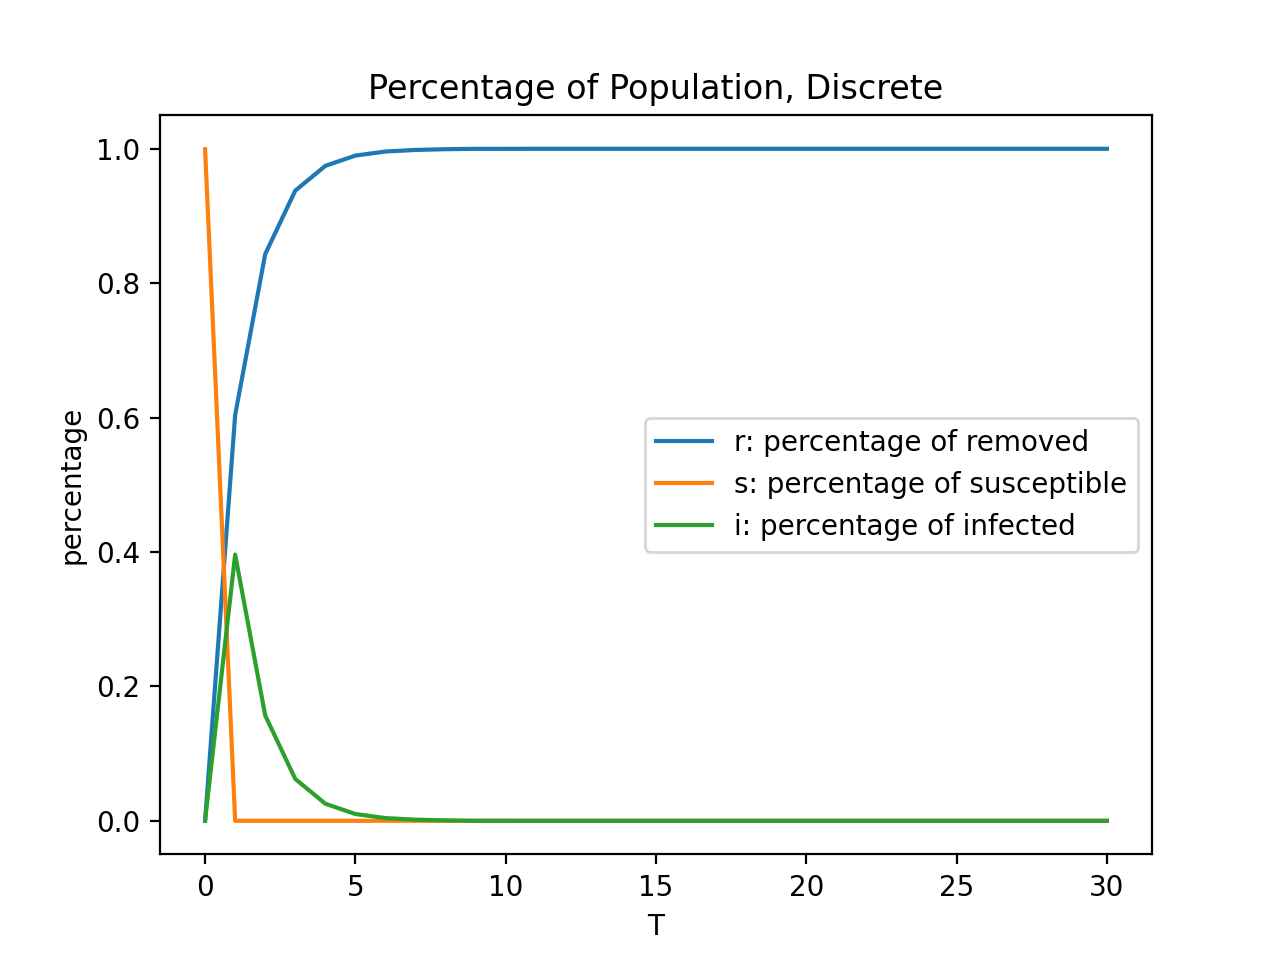
\includegraphics[width=.3\textwidth]{spatialagentsimulation.png}
\caption{Percentage of population susceptible (s), infected (i), and removed (r), Discrete}
\label{fig:figure1}
\end{figure}

Figure 1 is produced based on the simulated model as all the individuals start from the grid randomly. We set $k = 0.6$, $q = 0.08$, $p = 0.5$. We can see all the people will finally be infected which is reasonable since each individual will move with a large step size and radius for infecting susceptible people (0.08) is large as population size is 20000. We can observe that all susceptible people eventually get infected very quickly.



\subsubsection{Exploration on p and i}
Next, we explore the relationship between the total infected individuals and p as infected people initially located at the center of the confined region. We choose the parameters b = 0.5, k = 2 from the phase transition boundary.

\subsubsection{Exploration on p and i}
Next, we explore the relationship between the total infected individuals and p as infected people initially located at the center of the confined region. We choose the parameters b = 0.5, k = 2 from the phase transition boundary.

\begin{figure}[htp]
\centering
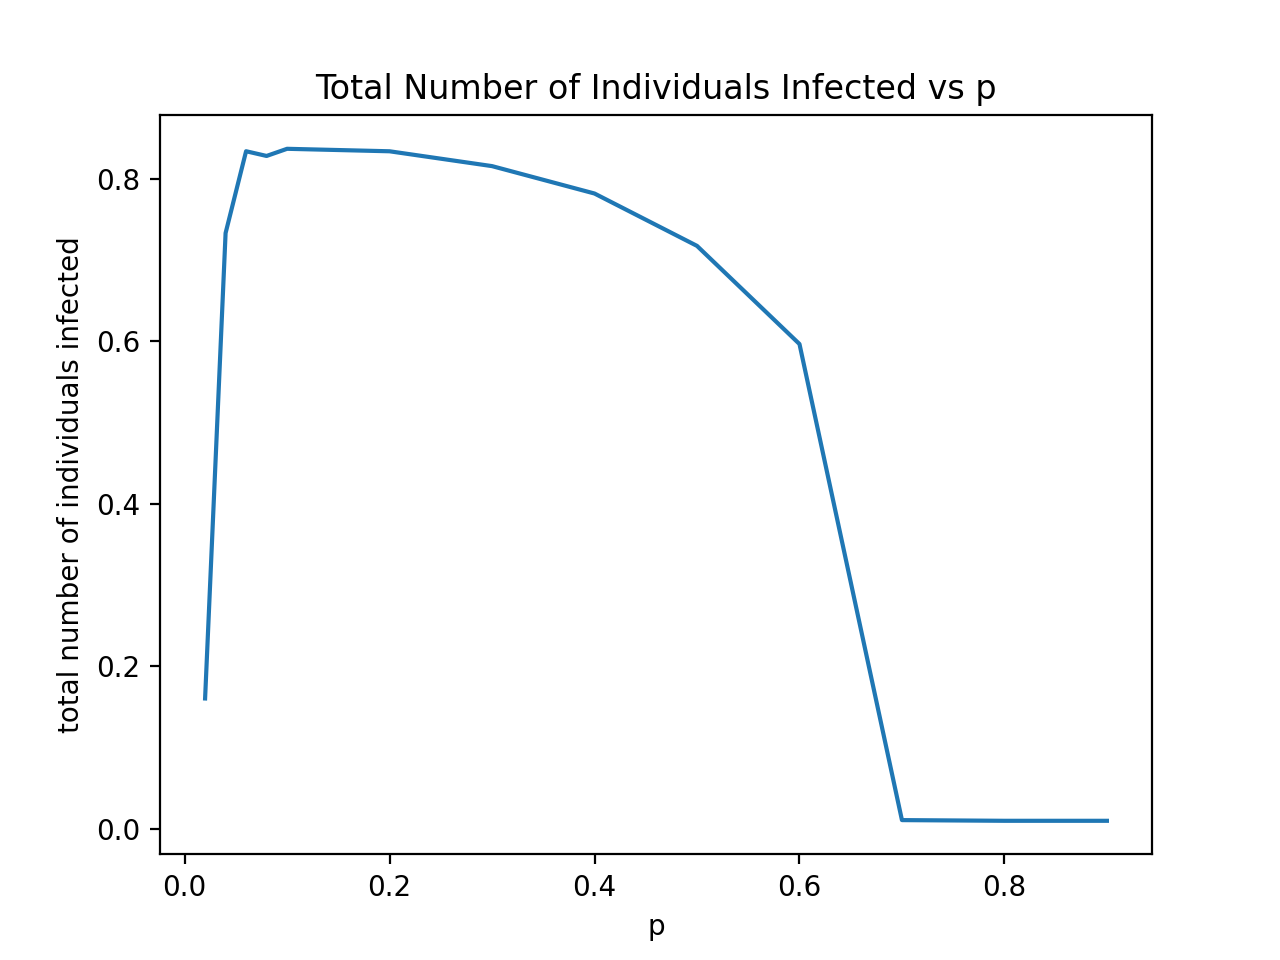
\includegraphics[width=.3\textwidth]{secondspatialplot.png}
\caption{Line plot for percentage of total infected individuals against p}
\label{fig:figure2}

\end{figure}


In figure 2, we can see that as p increases, the percentage of total infection increases until a peak value of around 0.8, which is reached at p = 0.1. Then, it remains stable as p changes from 0.1 to 0.2. As p increases from 0.2, the percentage of total infected decreases, and in particular it decreases sharply when $p > 0.7$.

The result of the plot matches our expectation. As p is small ($p=0.01$), initial infected individuals barely move. Only a small portion of susceptible people will get infected. People who are infected initially will be recovered and the total percentage of individuals infected is small. As $ 0.1<p<0.4 $, all the infected people will move around and contact most of susceptible people. The total percentage of infected people will be large. However, we choose the parameters b, k from transition boundary, and we can observe not all the people will finally be infected. As p is large, some of the infected people may stay at the original position because the step size is large. Thus, the total percentage of infected people will decrease. As p is extremely large, all the infected people will stay at the center. They can only infect the susceptible people around them initially. Hence, only small percentage of population will finally be infected.


Then, we discuss how the simulation qualitatively diffes when the initial infected individuals start in a single corner of the square vs. the center of the square vs. being randomly spread out. We choose the parameter p = 0.05. The conclusion is that the percentage of infected people will be 0.8522, 0.8098, 0.4994 as initial infected individuals start from random position, center, and corner respectively. We can see that the percentage of total infected will attain the maximum if all the infected people start from the random position in the grid. It will reach minimum if all the infected people start from a single corner of the grid. It is reasonable because as all the infected individuals move from a random position, they will frequently interact with different people among the population even the step size is small and it will be stable with most of people quickly get infected.

However, if all the infected people start from a single corner, they will not move too far away from that corner if the step size is small. Thus, they will only contact with a small amount of susceptible people and all the infected people will quickly be recovered. Thus, we conclude that total percentage of individuals infected will be small if they start from a single corner and the step size is small.

However, if all the infected people start from a single corner, they will not move too far away from that corner if the step size is small. Thus, they will only contact with a small amount of susceptible people and all the infected people will quickly be recovered. Thus, we conclude that total percentage of individuals infected will be small if they start from a single corner and the step size is small.

Next, we consider the case that all people start at the center with a small step size p = 0.05. Since infected people will contact with more people compared to the situation where they start at the corner, the total percentage of infected people will be larger. Nevertheless, the step size is small and all the infected people will also quickly be recovered. The total percentage of individuals infected will be smaller than the case that all the infected people are random spread out in the grid.






\subsection{Basic ODE Model}

We briefly introduced the ODE based model in the midterm checkpoint. The implementation is quite straightforward. The inputs for the derivative are three variables s, i, r and a function for obtaining derivative. Then we ran the ODE simulation with the solve ivp function. The result is reasonable and we almost have the same transition phase boundary as what we explored in the agent-based model. In the following part, we set the parameter b =1 and k = 0.4, and assume not all the people will be susceptible in this case.



\subsection{Spatial PDE Model}

\subsubsection{Implementation and Simulation}

We implemented the spatial PDE model by creating several functions to generate the desired distribution of population. The generatesum2 is the function for producing the population with initial infected people randomly spreaded out in the grid. The generatesum2center is the function for setting the infected individuals at center intially, while the generatesum2corner is the one setting the infected individuals at corner. We combined the s, i, r vector together as input for the derivative function, and then calculated the derivative according to the relationship:
$$\frac{\partial s(x,t)}{\partial t} = - b*s(x,t)*i(x,t) + p *L  s(x,t)$$

\noindent
As for $i(x,t)$ and $r(x,t)$, similar relationship could be established. Since we have the function for obtaining derivative, we can then simulate the PDE process.


\begin{figure}[htp]
\centering
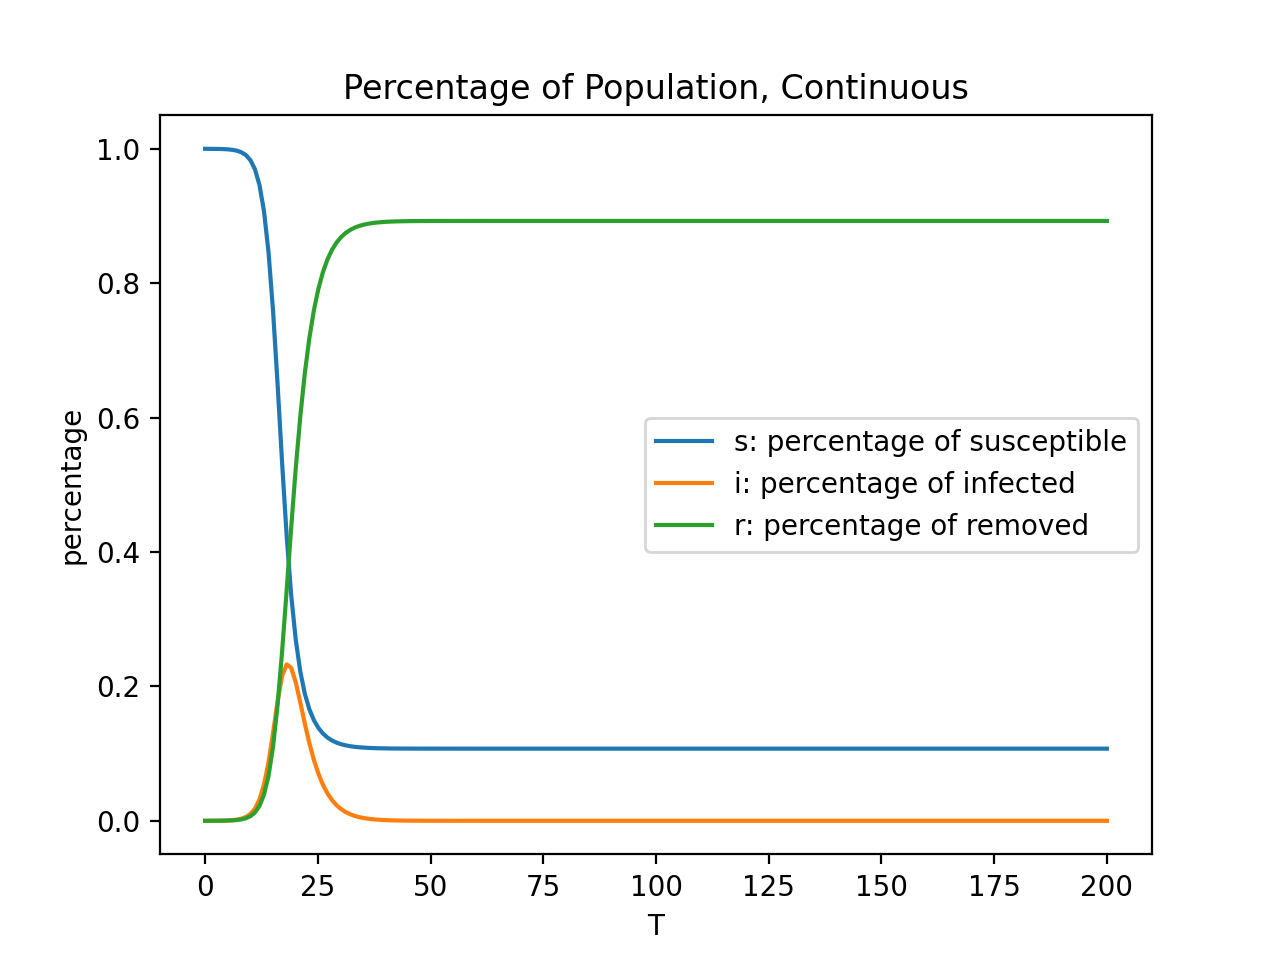
\includegraphics[width=.3\textwidth]{odesimulation1.png}
\caption{Percentage of population susceptible (s), infected (i), and removed (r), Continuous }
\label{fig:figure3}
\end{figure}
\FloatBarrier



Figure 3 shows reasonable result. Setting the parameter b=1 and k = 0.4, we observe the case that not all the individuals will finally be infected. We choose an appropriate diffusion term p = 1 so that all the susceptible in the grid can be potentially infected by the initially infected group located at center.



\subsubsection{Exploration on p and i}

In this section, we will analyze how the total percentage of infected people i changes with p. We choose the p in list $[1,2,3,4,5,10,20,30,40,50]$ with $b = 1$ and $k = 0.4$. Figure 4 suggests that as p increases, the percentage of total infected people will increase. The increment is not large.


\begin{figure}[htp]
\centering
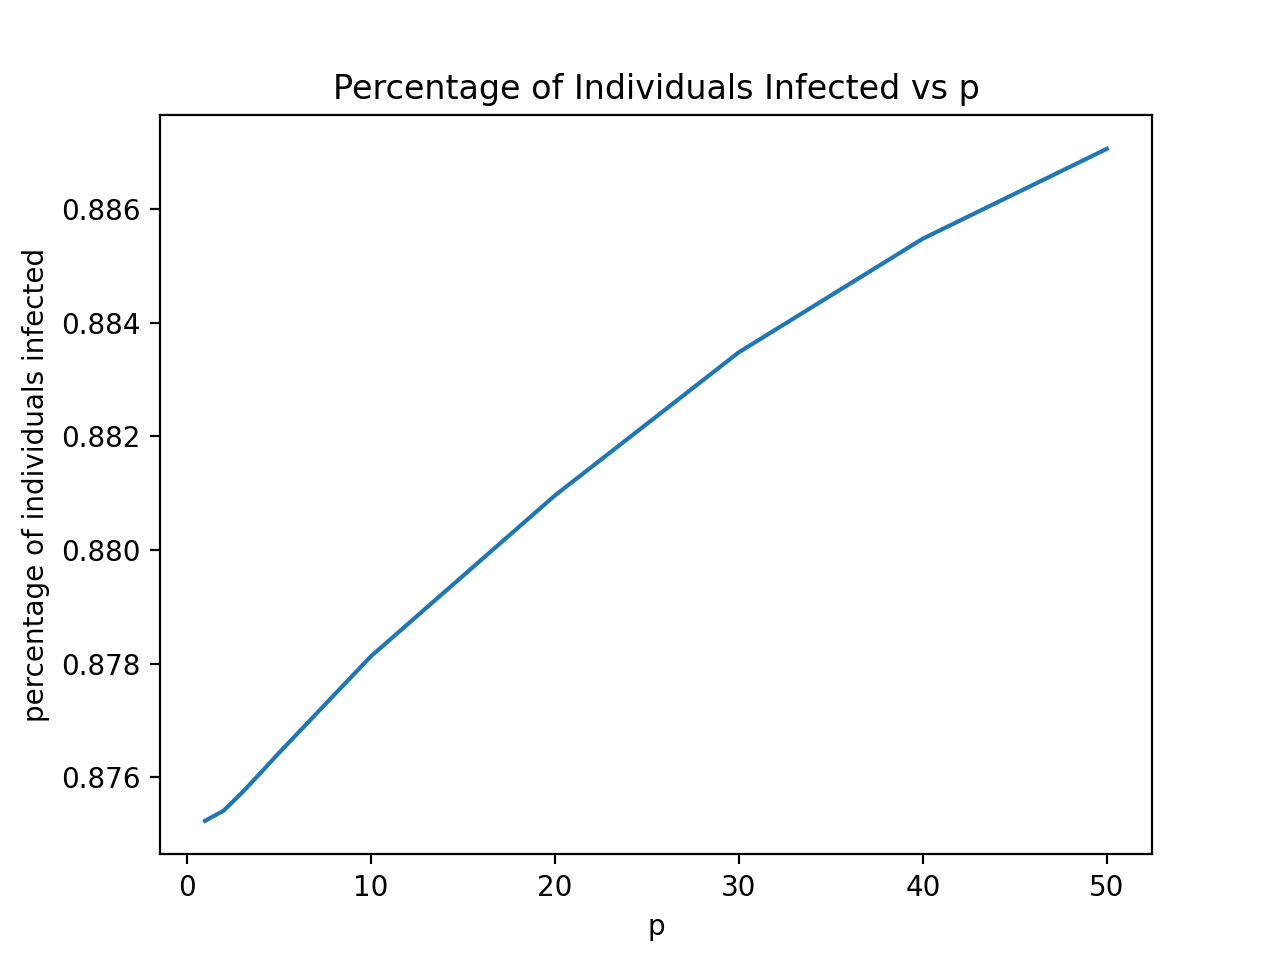
\includegraphics[width=.3\textwidth]{odeplot.png}
\caption{Line plot for percentage of total infected individuals against p, Continuous}
\label{fig:figure4}
\end{figure}
\FloatBarrier



 We can conclude that the percentage of total infected will be large if the diffusion term is large, since all the people will interact with individuals located in different positions frequently. The population will reach a stable state quickly. We also find that the increment is not large as p increases. This is because we have the diffusion term $p > =1$ which guarantees the condition that the infected people can be spread out in the grid before most of the infected people in population are recovered. Thus,as p is increasing, we can observe the increment while it is not large.



Then, we try to understand what will happen if we place infected people at different locations initially. As p = 20, the total infected percentage of population are 0.8926, 0.88, 0.86 as initial infected people are randomly spread out, located from center, located in a corner respectively. The result is reasonable. The total infected people will reach its maximum if people infected initially are distributed randomly in the grid because there is a chance that infected people may contact all the susceptible people in different positions before all the infected people are recovered. However, we control the relationship between b and k to ensure that not all the people will finally be infected. As for the case that all the infected people were initially located at center, we can see that the total percentage of infected people will be close to the first case since the diffusion term is large and most of infected people will have a chance to contact susceptible people before they are recovered. As for the case that all infected people were located at a corner initially, the total percentage of infected people will be smaller because the infected people will contact less people due to the starting position before they are recovered.



 \section{Modelling the Usage of Mask}

 \subsection{Modified SIR model with Mask}

We study the effectiveness of mask in the spreading of the novel COVID-19 disease and develop a variation of the SIR model that provides a theoretical framework to investigate its spread within a community. More specifically, we investigate how the usage of mask will influence the percentage of deaths and hospitalizations with respect to different infectious contact rate. The model is based on the paper "To mask or not to mask: Modeling the potential for face mask use by the general public to curtail the COVID-19 pandemic" by Steffen E. Eikenberry et al \cite{Steff2020mask}. In this model, we will introduce the variables S(t), E(t), I(t), H(t), A(t), R(t), and each denote susceptible, exposed, symptomatic infectious, hospitalized, asymptomatic infectious, and recovered classes, with an assumption that people progress from
$$S \rightarrow E \rightarrow A \rightarrow I \rightarrow H. $$

\noindent
The following is the equation for the mask simulation. We compare the case that most of  people wear mask with the case that people do not wear masks.

 \begin{minipage}{0.45\textwidth}
 \begin{eqnarray}
   \frac{dS}{dt} &=& -\beta{(t)}(I+\eta A)\frac{S}{N}\nonumber\\
   \frac{dE}{dt} &=& \beta(t)(I+\eta A)\frac{S}{N}-\sigma{E}\nonumber\\
   \frac{dI}{dt} &=& \alpha\sigma{E}-\phi{I}-\gamma_{I}I\nonumber\\
   \frac{dA}{dt} &=& (1-\alpha)\sigma E-\gamma_{A}A\nonumber\\
   \frac{dH}{dt} &=& \phi I - \sigma H - \gamma_{H}H\nonumber\\
   \frac{dR}{dt} &=& \gamma_{I}{I} + \gamma_{A}{A}+\gamma_{H}{H}\nonumber\\
   \frac{dD}{dt} &=& \sigma H\nonumber\\
 \end{eqnarray}
 \end{minipage}
 \begin{minipage}{0.35\textwidth}
 \tiny
 \begin{eqnarray}
   \frac{dS_{U}}{dt} &=& -\beta(I_{U}+\eta A_{U})\frac{S_{U}}{N}-\beta((1-\epsilon_{0})I_{M}+(1-\epsilon_{0})\eta A_{M})\frac{S_{U}}{N}\nonumber\\
   \frac{dE_{U}}{dt} &=& \beta(I_{U}+\eta{A}_{U})\frac{S_{U}}{N}+\beta((1-\epsilon_{0})I_{M}+(1-\epsilon_{0})\eta A_{M}))\frac{S_{U}}{N}-\sigma E_{U}\nonumber\\
   \frac{dI_{U}}{dt} &=& \alpha\sigma E_{U}-\phi I_{U} - \gamma_{I}I_{U}\nonumber\\
   \frac{dA_{U}}{dt} &=& (1-\alpha)\sigma E_{U}-\gamma_{A}A_{U}\nonumber\\
   \frac{dH_{U}}{dt} &=& \phi I_{U}-\delta H_{U}-\gamma_{H}H_{U}\nonumber\\
   \frac{dR_{U}}{dt} &=& \gamma_{I}I_{U}+\gamma_{A}A_{U}+\gamma_{H}H_{U}\nonumber\\
   \frac{dD_{U}}{dt} &=& \delta H_{U}\nonumber\\
   \frac{dS_{M}}{dt} &=& -\beta (1-\epsilon_{i})(I_{U}+\eta A_{U})\frac{S_{M}}{N}-\beta(1-\epsilon_{i})((1-\epsilon_{0})I_{M}+(1-\epsilon_{0})\eta A_{M})\frac{S_{M}}{N}\nonumber\\
   \frac{dE_{M}}{dt} &=& \beta(1-\epsilon_{i})(I_{U}+\eta A_{U})\frac{S_{M}}{N}+\beta(1-\epsilon_{i})((1-\epsilon_{0})I_{M}+(1-\epsilon_{0})\eta A_{M})\frac{S_{M}}{N}-\sigma E_{M}\nonumber\\
   \frac{dI_{M}}{dt} &=& \alpha\sigma E_{M}-\phi I_{M}-\gamma_{I} I_{M}\nonumber\\
   \frac{dA_{M}}{dt} &=& (1-\alpha)\sigma E_{M}-\gamma_{A}A_{M}\nonumber\\
   \frac{dH_{M}}{dt} &=& \phi I_{M}-\delta H_{M}-\gamma_{H} H_{M}\nonumber\\
   \frac{dR_{M}}{dt} &=& \gamma_{I}I_{M}+\gamma_{A}A_{M}+\gamma_{H}H_{M}\nonumber\\
   \frac{dD_{M}}{dt} &=& \delta H_{M}\nonumber\\
   \end{eqnarray}
 \end{minipage}






 \subsection{Implementation}

 We ran the simulation and recorded what happened in several days. Here, $\beta $ is the infectious contact rate, $\sigma $ is the transition exposed to infectious, $\eta $ is the infectiousness factor for asymptomatic carrier, $\alpha$ is the fraction of infections that become symptomatic, $\phi$ is rate of hospitalization, $\gamma_{A}$ is the recovery rate for asymptomatic, $\gamma_{I}$ is the recovery rate of  symptomatic, $\gamma_{H}$ is the recovery rate for hospitalized, $\sigma$ is the death rate in hospital, $\epsilon_{0}$ is the outward efficiency of the masks, while $\epsilon_{I}$ is the inward efficiency of the masks. Then we found the default estimated values for all parameters with population masked and not masked from the paper \cite{Steff2020mask}. Firstly, we ran the case of simulation that people do not wear mask, and added several factors mentioned above. Figure 5 shows that the general trend of simulation is very similar to the SIR simulation. We will regard this as the base case.


 \begin{figure}[htp]
 \centering
 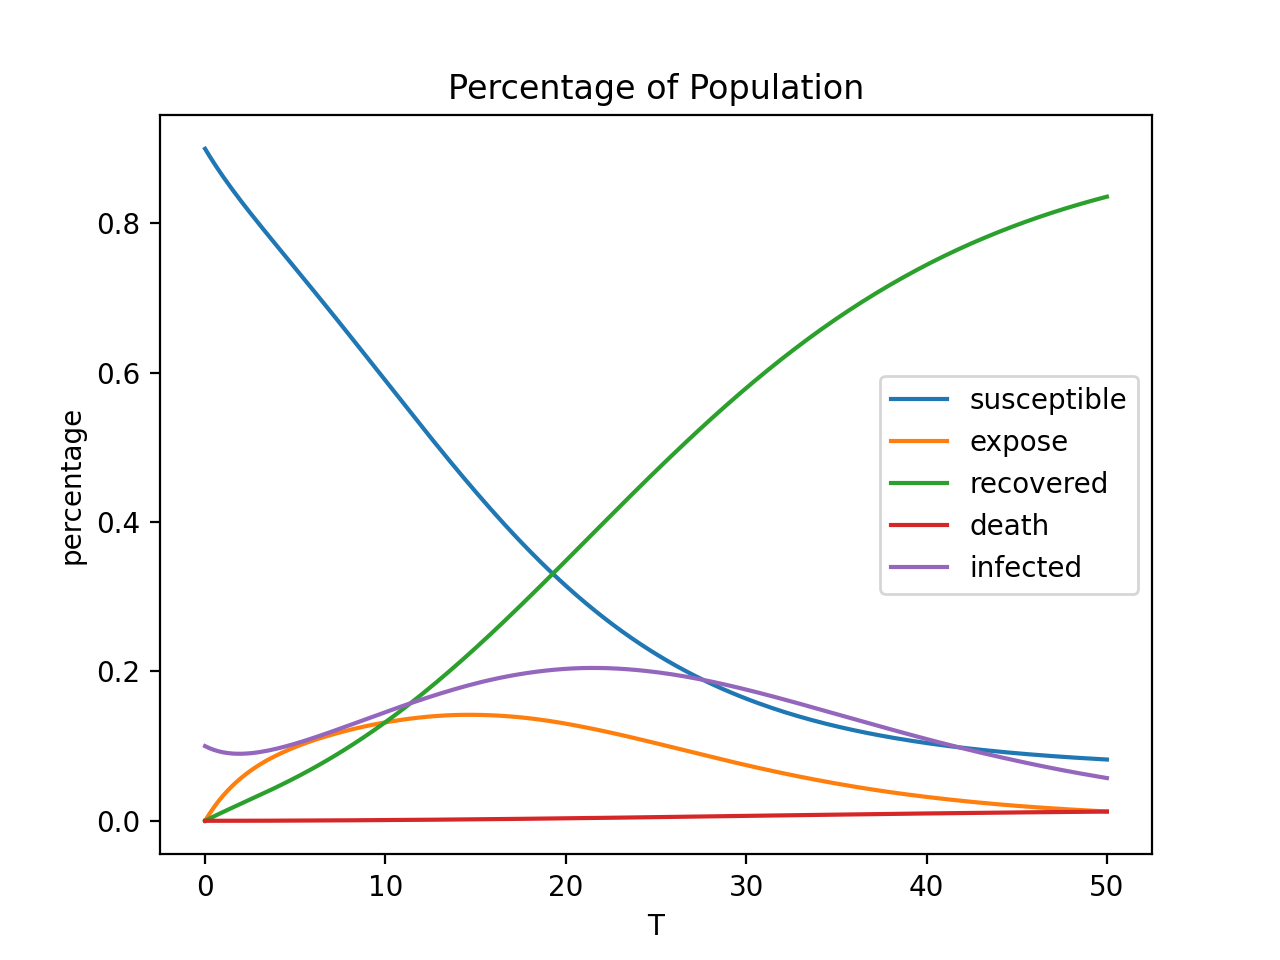
\includegraphics[width=.3\textwidth]{masksimulation.png}
 \caption{no mask simulation}
 \label{fig:figure5}
 \end{figure}

Then, we ran the simulation for the case that people wear masks.
Here, an assumption was made that the inward efficacy and outward efficacy of masks are the same $\epsilon_{0} = \epsilon_{1}$. We drew a 2 dimensional phase diagram to show how the efficacy of mask (homemade mask or surgery mask) and the percentage of masked people would influence the rate of peak hospitalization as well as the rate of total deaths among the population.


\begin{figure}[htp]

\centering
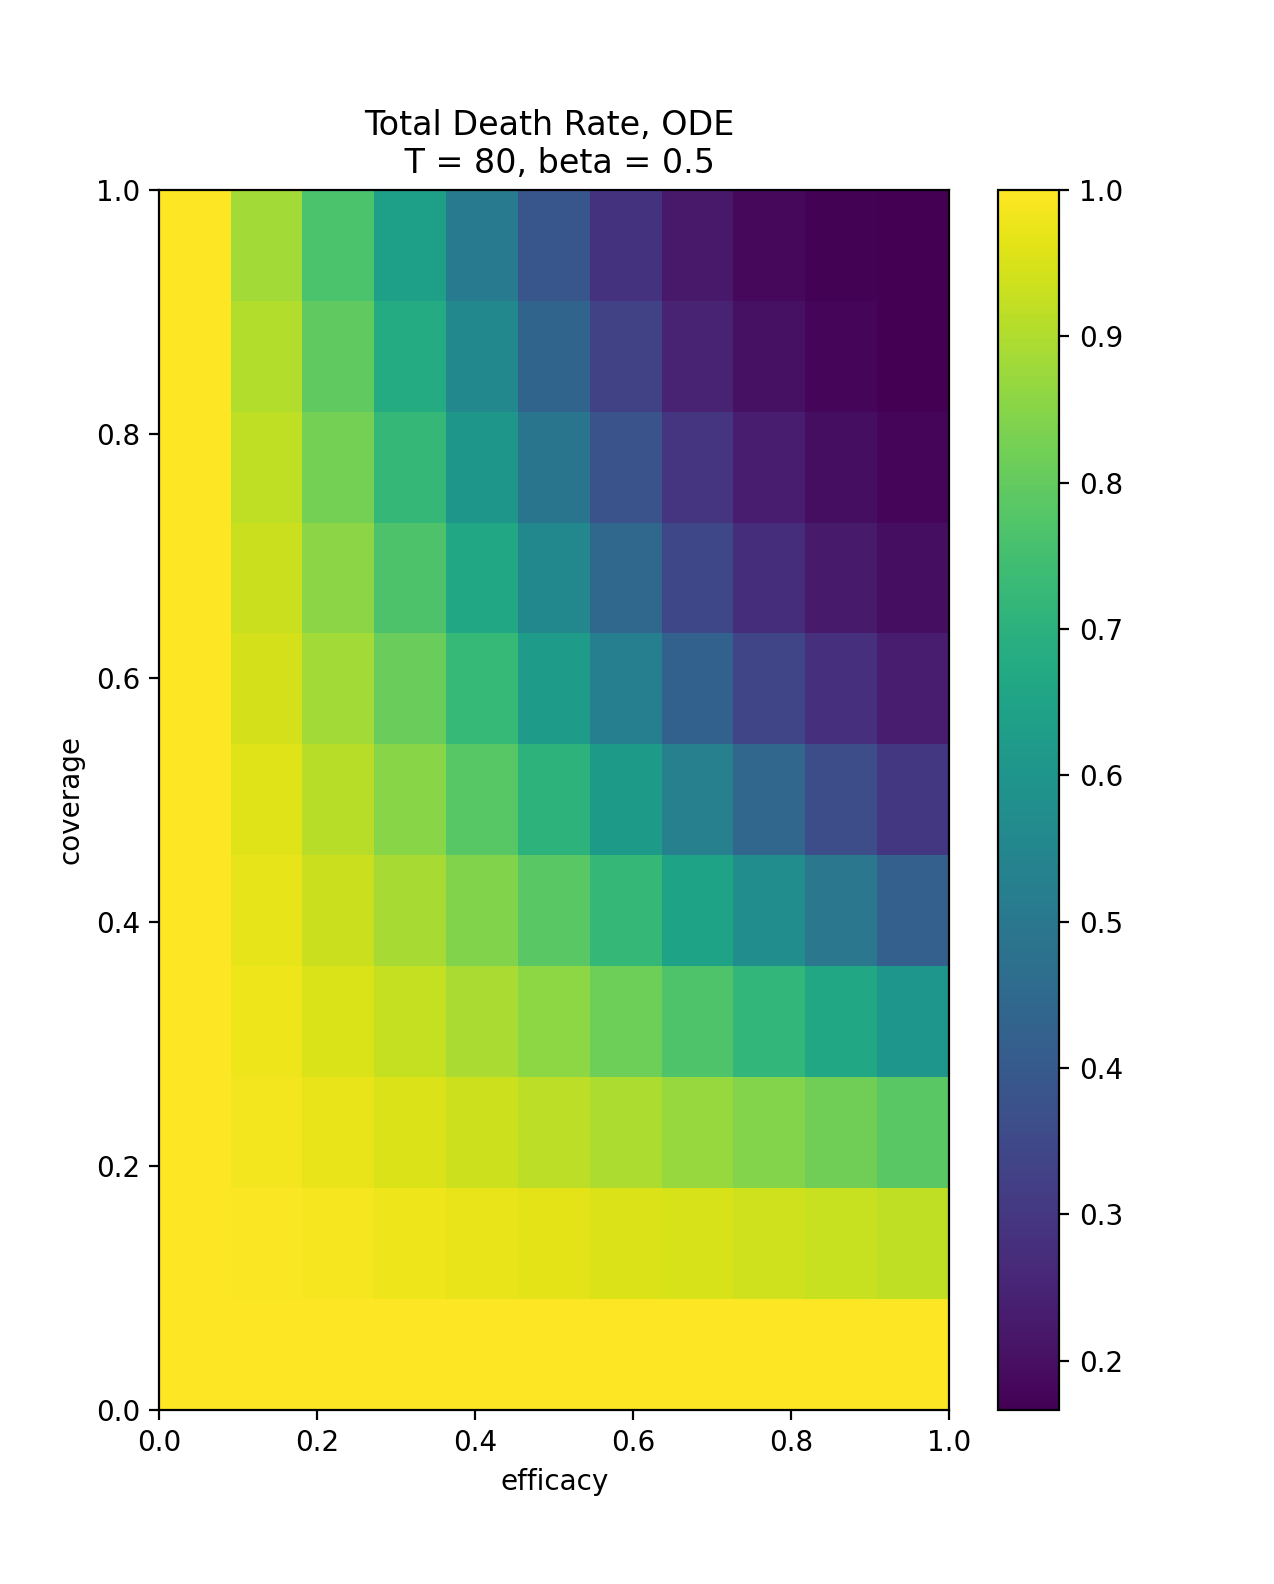
\includegraphics[width=.2\textwidth]{death0.5.png}\hfill
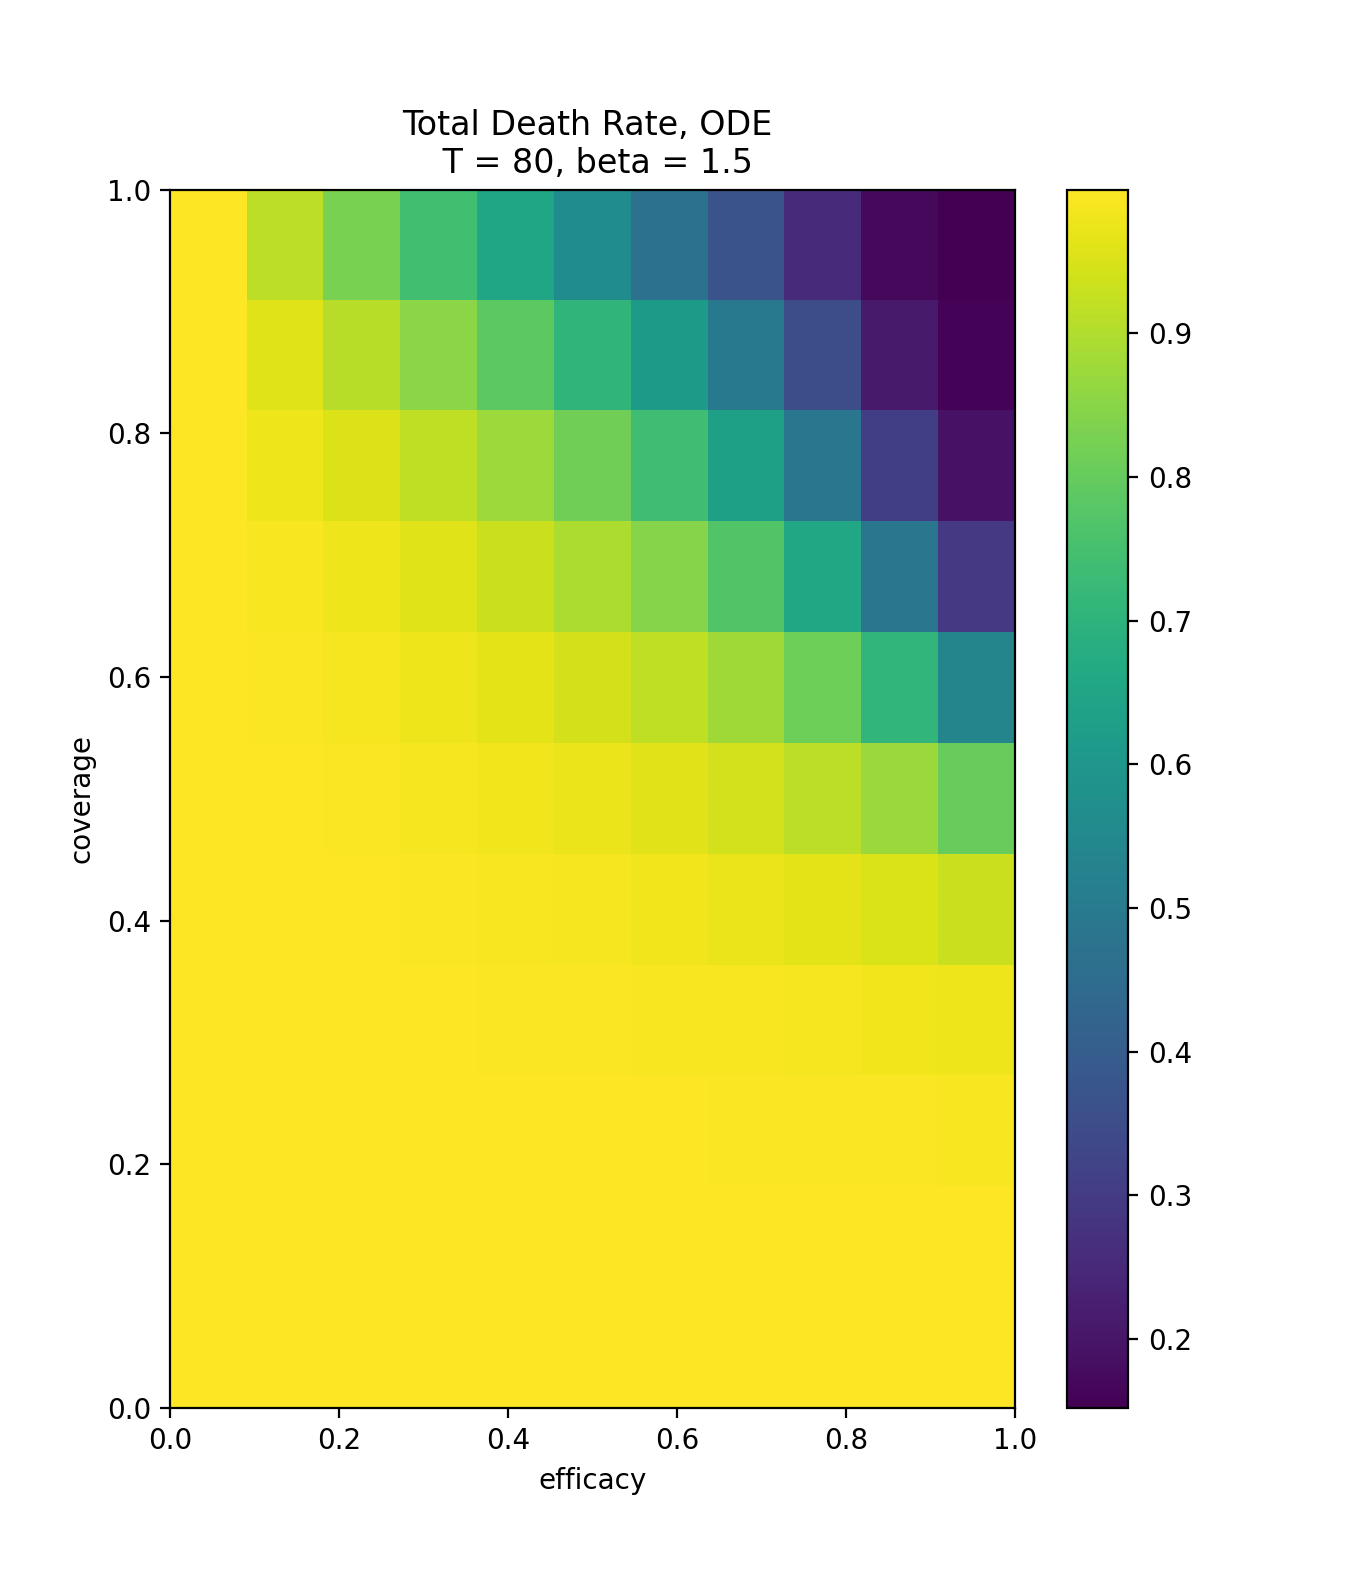
\includegraphics[width=.2\textwidth]{death1.5.png}\hfill
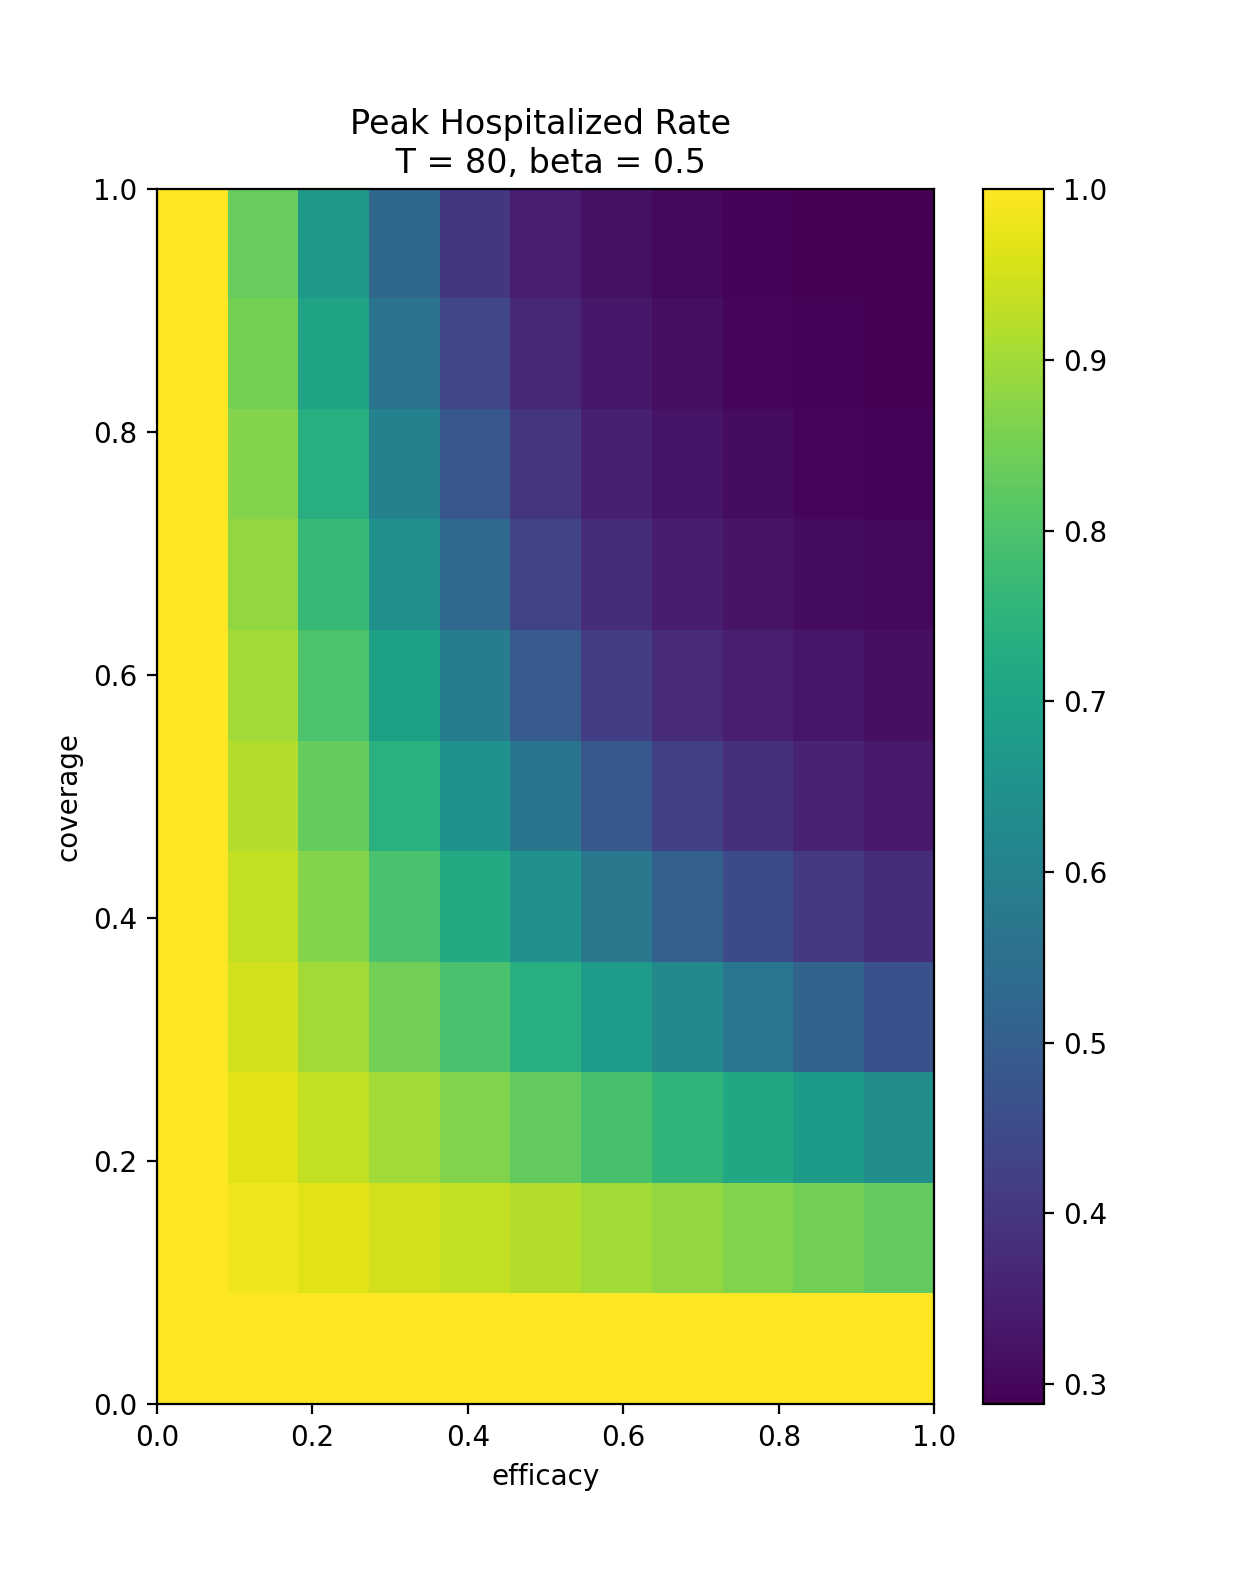
\includegraphics[width=.2\textwidth]{hospital0.52.png}\hfill
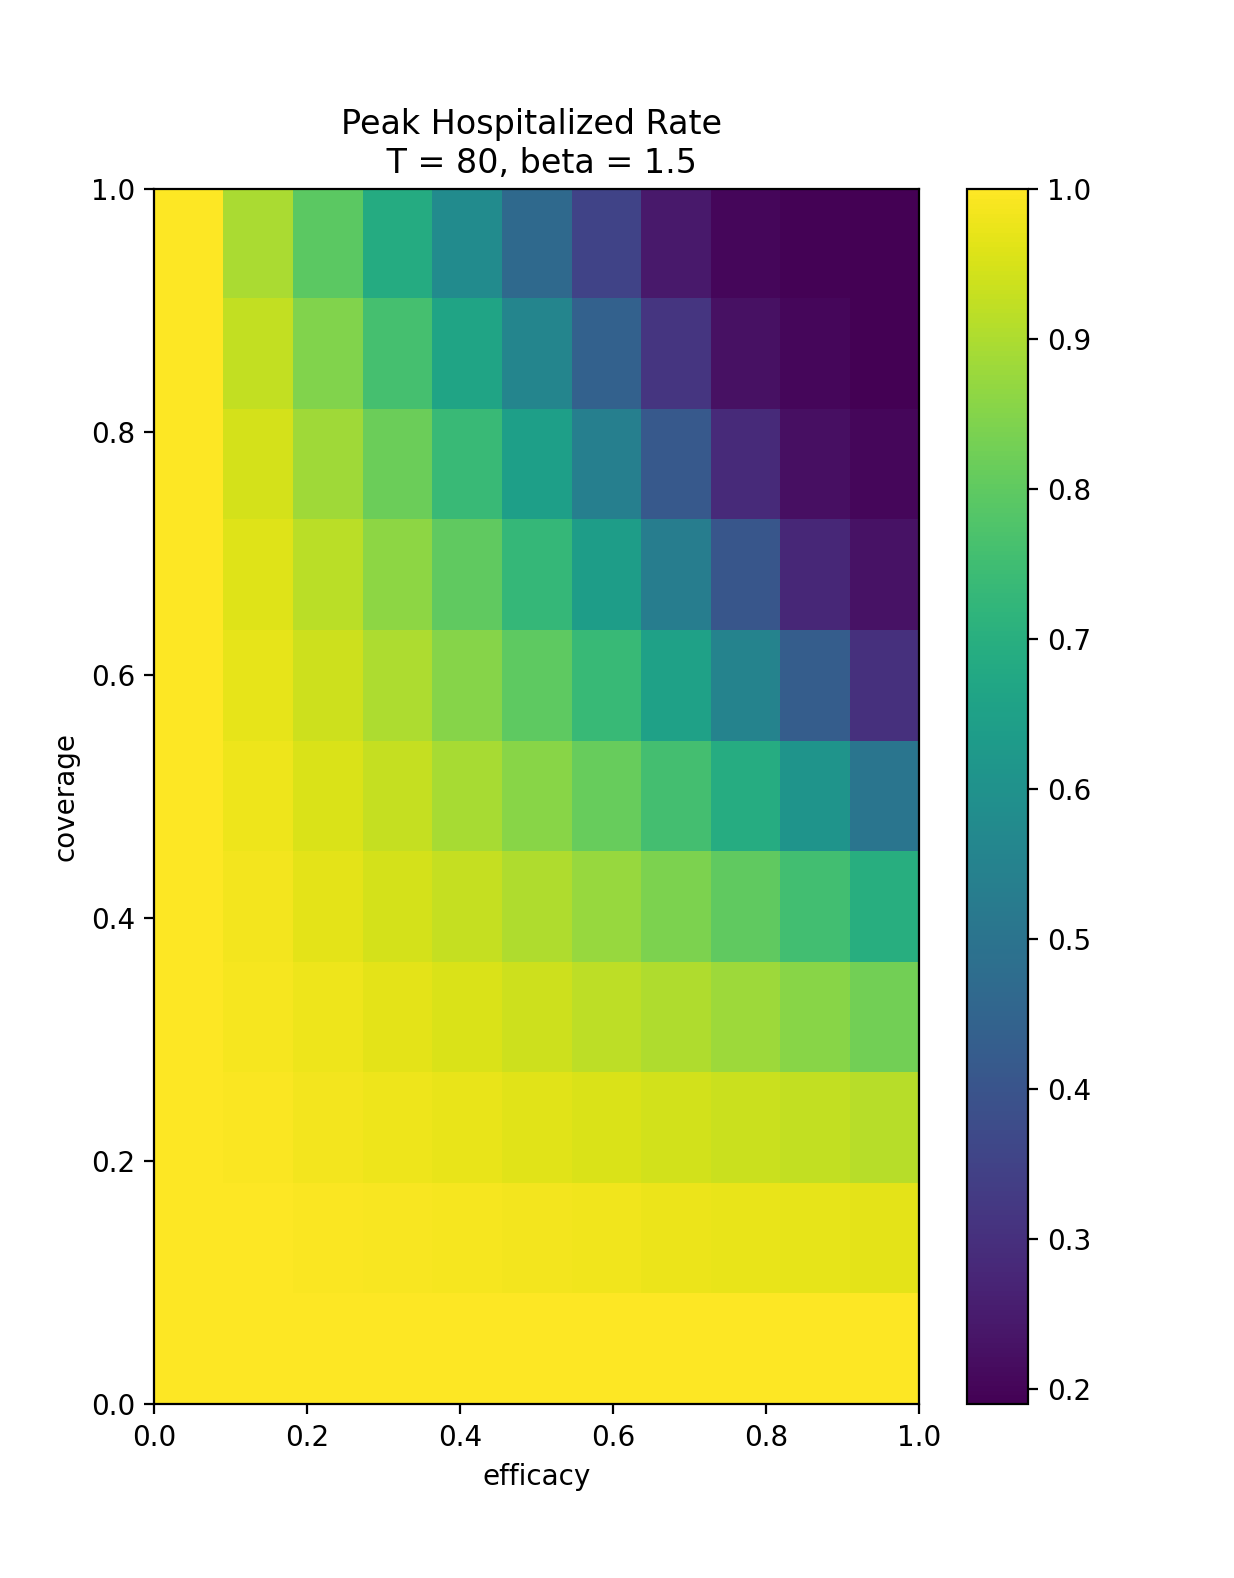
\includegraphics[width=.2\textwidth]{hospital1.52.png}

\caption{Phase diagrams for mask efficacy and coverage}
\label{fig:figure6}

\end{figure}







\subsection{Results and Discussion}

Figure 6 shows the relative peak hospitalizations and cumulative mortality under simulated epidemics, $\beta = 0.5$ or $\beta = 1.5$. When $\beta$ is large, it is the only case that large amounts of people wearing high efficacy mask can prevent the transmission of virus. These results are relative to the case where no masks are used. From the phase diagrams presented, we observe asymmetry between coverage and efficacy, and increasing the coverage of moderately effective mask is generally more useful than increasing the efficacy of masks from a starting point of moderate coverage. The results agreed with the one concluded from the paper. Therefore, these findings suggest that face mask should be adopted as early and universal as possible, even if most masks are not highly effective.


Yet, there are some limitations in our model. Since we used default values based on the source paper\cite{Steff2020mask}, it may not match with the situation in reality, which can be improved. Furthermore, we assumed that the inward and outward efficacy are same, which might not be true in practice, and the values could be improved with more detailed and carefully designed research and study.






\section{Fitting Covid-19 data with SIR model}

\subsection{Introduction and Implementation}

In this variation, we will fit the SIR model with the Covid-19 dataset in China Hubei Province. Instead of using the SARS data set claimed in midterm report, we find that Covid-19 dataset in China is complete.

We collect the data set from \cite{Johnhopkins} in first 76 days. The Covid-19 was controlled in China in around 76 days. Building the specialized hospital helped the government to collect severe patients so that the transmission of Covid-19 was controlled. We divided the process of simulation in two phases. First, people were not aware that Covid-19 is a kind of coronavirus which can severely influence life. After around 25 days of pandemic period, the government started to control the Covid-19 through building large hospitals for collecting severe patients and announced the policy that all the people should stay at home, especially in Hubei. From then on, the total infected people were stable after around 50 days. We try to simulate the whole process through the basic SIR model.

In the first phase, we use the default parameters from the source \cite{Cooper2020SIR} $b = 0.35$ and $r = 0.03$. We explore a range of b, k parameters so that in first 25 days, the MSE of the i, r people in Hubei and the simulated i, r values will attain the minimum. We use the function calculate MSE between the simulated value and practical data set. We conclude that in first phase, $b = 0.23$ and $k = 0.025$.

As for the second phase, we apply the same function to find the most appropriate b, k according to MSE between simulated data and real data set. However, the policy is adjusted here and most of infected people are moved to hospitals, the transmission rate b will be much smaller than original value. We try to find b from the range $[0.01, 0.04]$ and it works. We get $b_{2}= 0.02$, and $k_{2} = 0.06$. The result is reasonable compared with the default value in the paper \cite{Cooper2020SIR}. The recovered rate should be around 0.05 per infected person each day. As people recognized the fact that Covid-19 is a severe coronavirus, most people started wearing masks and stayed at home. Even if they were infected with Covid-19, the chance of being recovered was improved.





\subsection{Results and Discussion}

From figure 7, we can see that the observed curve is close to the real data set with small deviation. There are several reasons that the simulated curve is not very close to the real data set. First of all, the SIR model is a little bit simplified. To be specific, we do not consider the case that some people may be asymptomatic among the population. The recover rate and hospitalized rate are different for asymptomatic group and symptomatic group. The SIR model does not take account into these variations.


\begin{figure}[htp]
\centering
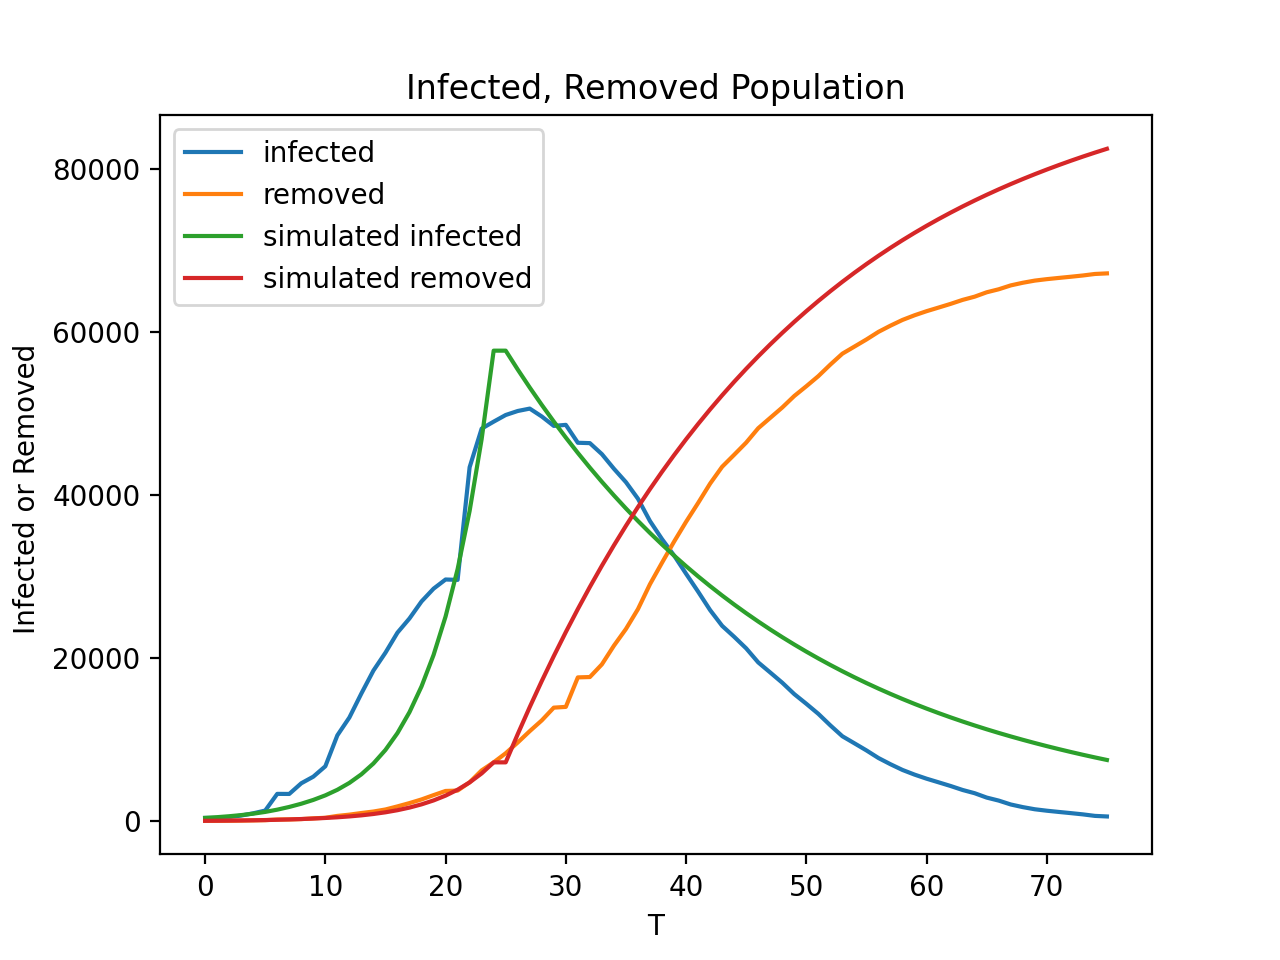
\includegraphics[width=.3\textwidth]{covidsir4.png}
\caption{covid-19 data fit}
\label{fig:figure6}
\end{figure}



Apart from that, the limitation comes from the incomplete statistics. For a large province in China, it is hard to ensure the data set is matched with the real case. Some infected people may not be tested as positive while the tested sample is only part of the population.


Finally, there is also some possibility that the factors influencing Covid-19 is hard to be identified. For instance, we regard the transmission rate and recovered rate as constant in two phases. However, the transmission rate or recovered rate may change frequently in several weeks due to the change of climate or some other factors. We will get more accurate results if we have enough research related to Covid-19. We can take action if we recognize winter or spring is appropriate for the virus to be spread among the population.


To be summarized, we conclude three factors that may influence our simulation include the over-simplified SIR model, the incomplete statistics and complex factors influencing transmission of Covid-19. We can run an accurate simulation if we have a more complex model taking into account different groups among the population, having a method for collecting the complete sample for recovered or confirmed individuals, or recognizing what exactly influenced the spread of Covid-19 after some researches. However, recognizing the policy announced from government during the process of controlling the transmission of Covid-19, we may simulate the result with a basic SIR model and adjust relevant parameters to fit the model.










\section{Data Visualization of Covid-19 in US}

The year 2020 has been dominated by the coronavirus disease 2019 (Covid-19) over the world. In this section, we will take an updated look at how the pandemic progressed thus far in the United States.


In order to explore the trend and distribution in terms of Covid-19 in the United States, we generated some interactive plots to provide better visualization and detailed information. The data sets are from the data repository for the 2019 Novel Coronavirus Visual Dashboard operated by the Johns Hopkins University Center for Systems Science and Engineering (JHU CSSE) \cite{Johnhopkins}, and we mainly used the daily time series summary table, including confirmed, deaths and recovered in US from January to present. The package `bokeh` is an interactive visualization library for modern web browsers, and the passive inspector tool called hover was added on to display the informational tooltips \cite{bokeh}.


First of all, we made the time series plots to reflect the cumulative trend of confirmed cases and deaths of Covid-19 for all states, and we observed that the trends increased over time for all states, which revealed the serious situation of Covid-19 in US. In figure 8, California, Texas, and Florida are the top three states with most confirmed cases, while Illinois and New York are following the next. Overall, the states with larger population have much more confirmed cases than the other states. Another interesting finding is that the confirmed cases increases dramatically first in New York during April, and tends to slow down from May to October, but recently the increase rose enormously again. The rapid growth of confirmed cases in Illinois from October might be the reason for the Executive Order 2020-10 issued by Governor Pritzker which stated all individuals should stay at home. As for the cumulative deaths, figure 8 shows that New York has the most deaths over time, and the states with larger population tends to have more deaths.





\begin{figure}[htp]
\centering
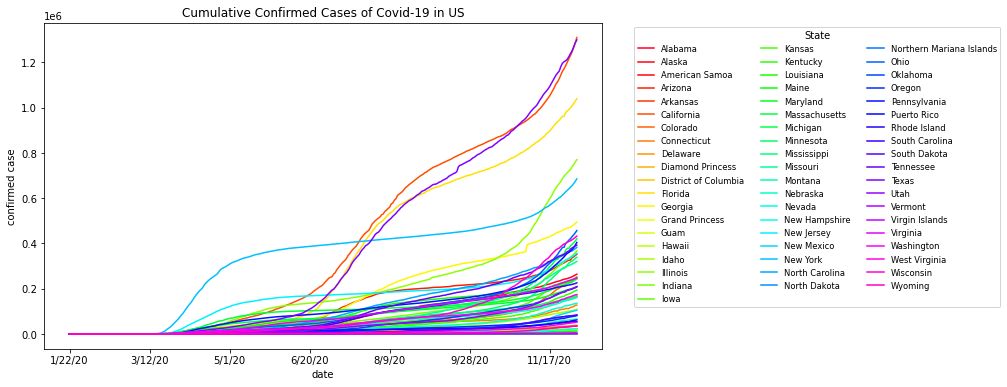
\includegraphics[width=0.5\textwidth]{cum_confirmed2.png}\hfill
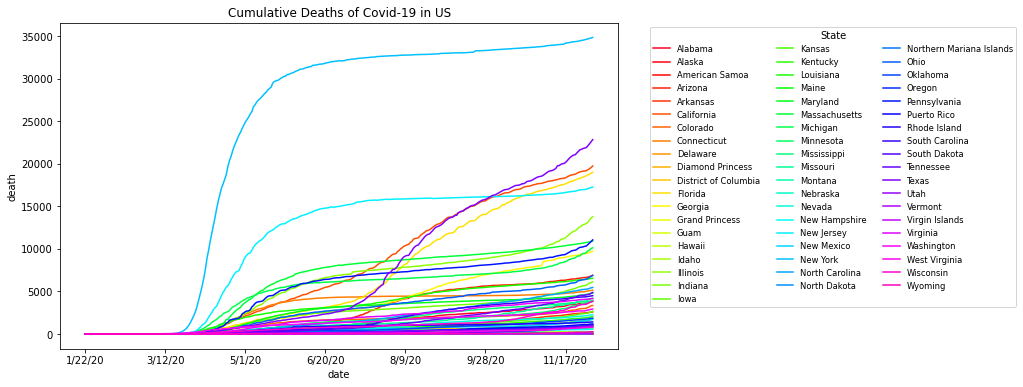
\includegraphics[width=0.5\textwidth]{cum_death2.png}
\caption{Cumulative confirmed cases and deaths of Covid-19 from 1/22/2020 to 12/4/2020 for all states in US}
\label{fig:figure}

\end{figure}
\FloatBarrier




\subsection{Interactive Time Series Plot}

\subsubsection{Implementation}


To improve the visualization and offer clear information, the interactive times series plots of daily confirmed cases of Covid-19 were generated using the `bokeh` package. We added the hover tooltips to provide the state name, the confirmed cased and the date, moving the mouse along the trends.


Since it was hard to observe the trends of all states in one plot, we decided to separate the states into four groups according to their locations: the Northeast, the Midwest, the South, and the West \cite{USregion}. We would select a few of states to represent each group. The Northeast includes Maine, New Hampshire, Vermont, Massachusetts, Rhode Island, Connecticut, New York, New Jersey, and Pennsylvania. We chose the states on West Coast to represent the West: California, Oregon, Washington, and Alaska, and chose six states of the Midwest: Ohio, Michigan, Indiana, Illinois, Missouri, and Nebraska. The South claims more states, and eight of them were selected: Delaware, Maryland, Virginia, Tennessee, Georgia, Florida, Mississippi, and Texas. The plot HTML's are stated in Appendix.



\subsubsection{Results and Discussion}


In figure 9, the plot for Northeast illustrates there are 11434 confirmed cases in New York on April 15, and the number of infected individuals are very large in April. New York is one of the worst-affected states in the United States. Moreover, the confirmed cases in Pennsylvania increases enormously in recent days and reaches to 12087 cases in one day on December 4. For the Midwest, Illinois, Michigan and Ohio are the three states with large population that show huge increases of confirmed cases recently. We observe similar trends of Texas and Florida in the South plot that have the first wave of confirmed cases around July and then the second wave in recent months. Along the west coastline, California takes the largest daily confirmed cases as well as the cumulative cases. On December 4, it has 23757 new confirmed cases, which is extremely horrible. It appears that the second wave is going to come with a much higher peak than the first one in summer.


From all four plots in figure 9, we notice that during the summer many states had a respite from Covid-19 with the fairly stationary trends of daily confirmed cases, except Florida, Texas and California whose population was overflowed. However, as the temperature drops the confirmed cases starts picking back up and almost all states show clear increasing trends. We may expect the Covid-19 to be seasonal like the flu, but the data set is not sufficient to give evidence. Furthermore, more time series analysis of Covid-19 should be done for future study, including fitting models (MA, AR, ARIMA, etc.) and predicting the future trend.



Figure 10 shows the daily deaths for four regions. It is not surprising that New York had the a large number of deaths in April, since people did not realize the severeness of Covid-19 at that time. It reached the highest number of deaths on April 7. The good thing is that the trends of deaths decrease quickly and move forward with relatively low values. For the Midwest, Illinois and Michigan are still the worst two states with higher number of deaths. What is even worse is that the trend of deaths demonstrate a sign of increase recently. Similarly, Texas and Florida are outstanding in the South with larger deaths than the rest of states. Moreover, California has larger variance than the other states on West Coast. Its trend can be considered as stationary over time.


\begin{figure}[H]
\centering
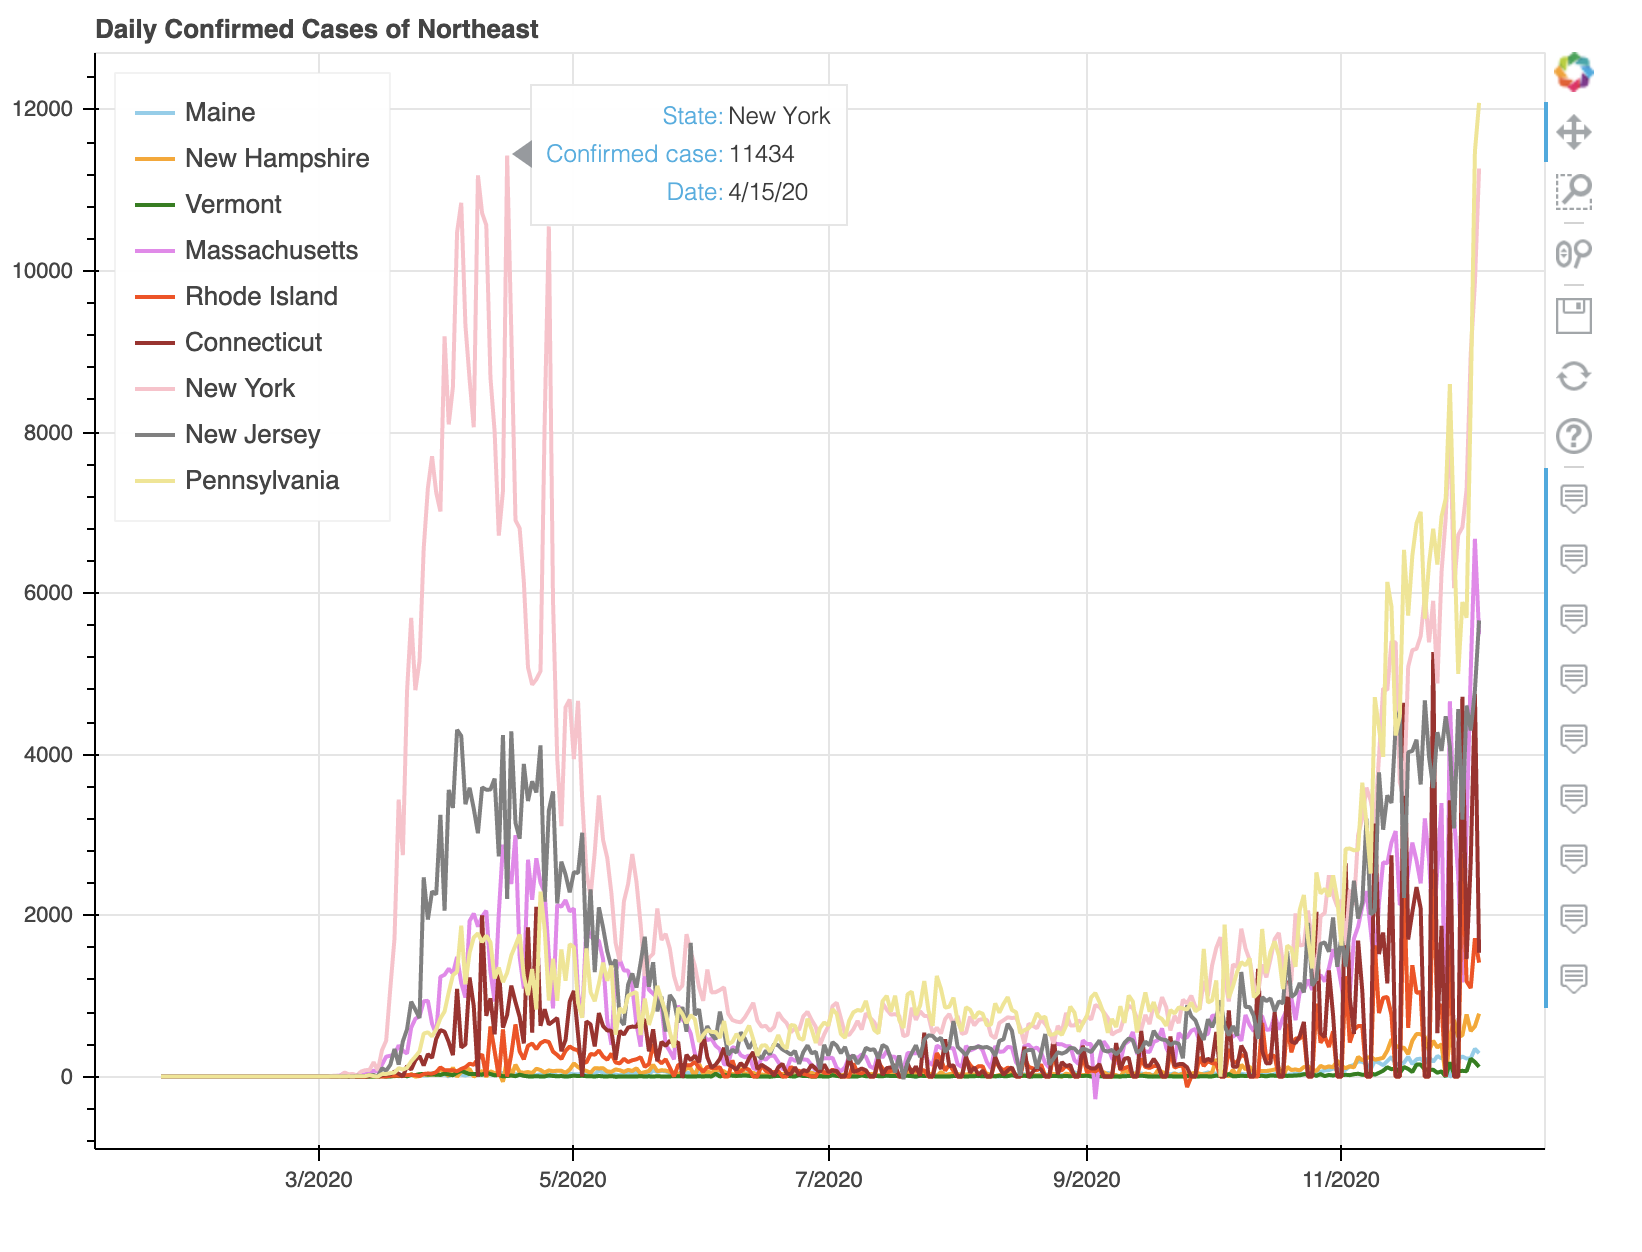
\includegraphics[width=.4\textwidth]{ts_northeast.png}
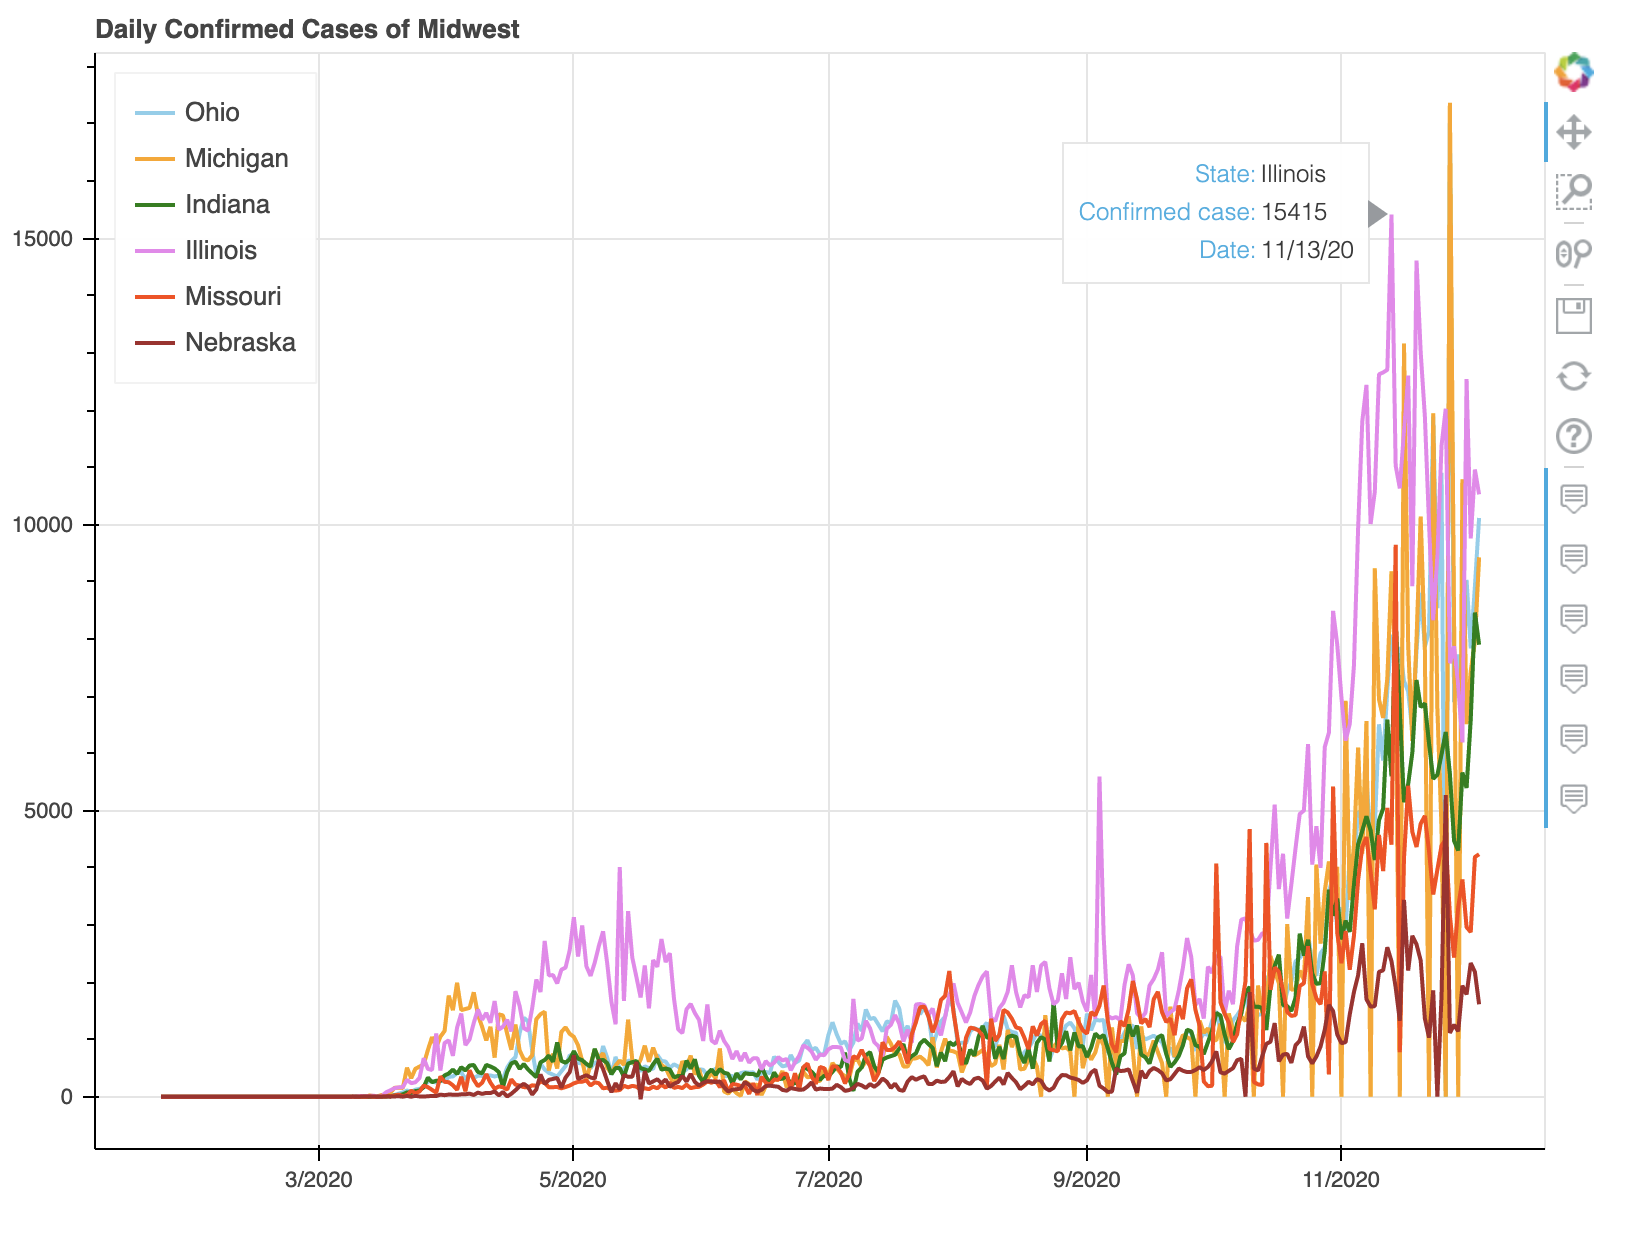
\includegraphics[width=.4\textwidth]{ts_midwest.png}
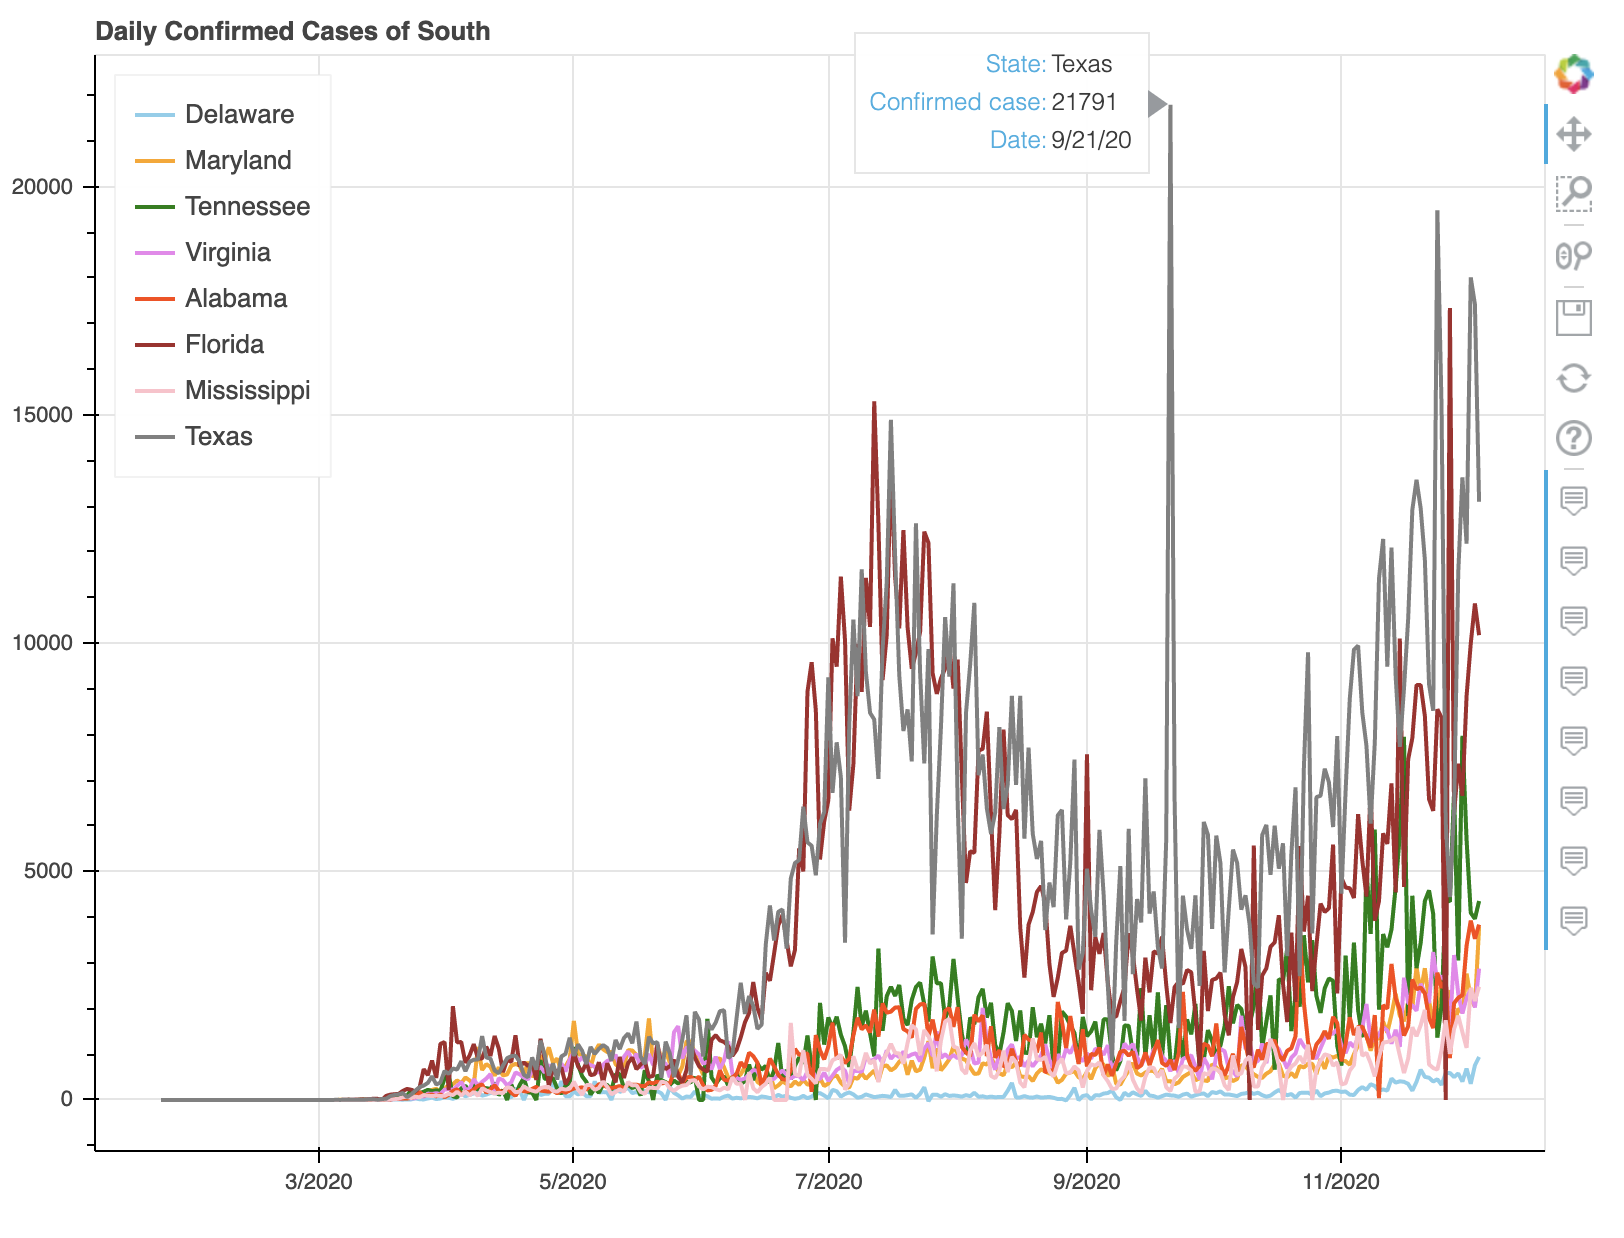
\includegraphics[width=.4\textwidth]{ts_south.png}
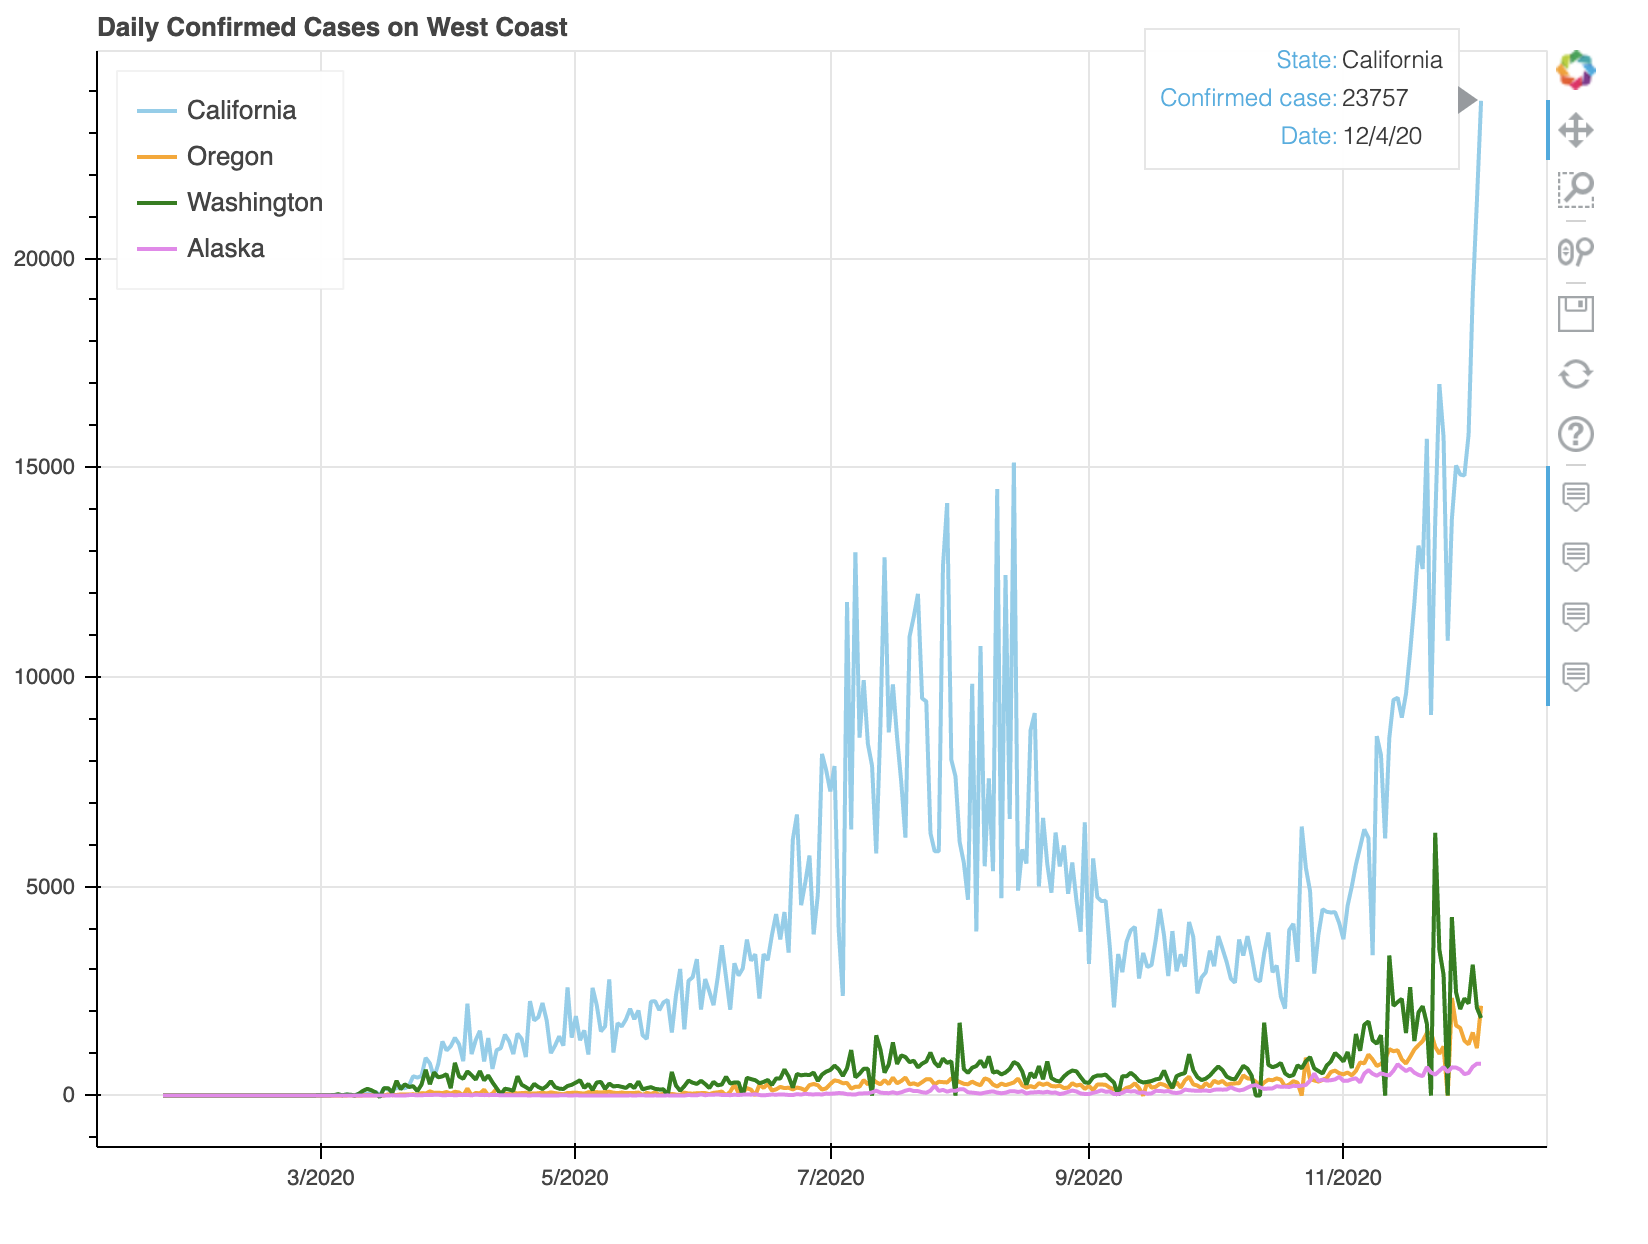
\includegraphics[width=.4\textwidth]{ts_west.png}

\caption{Interactive time series plots of daily confirmed cases of Covid-19 from 1/24/2020 to 12/4/2020 for states in US}
\label{fig:figure}
\end{figure}
\FloatBarrier


\begin{figure}[htp]

\centering
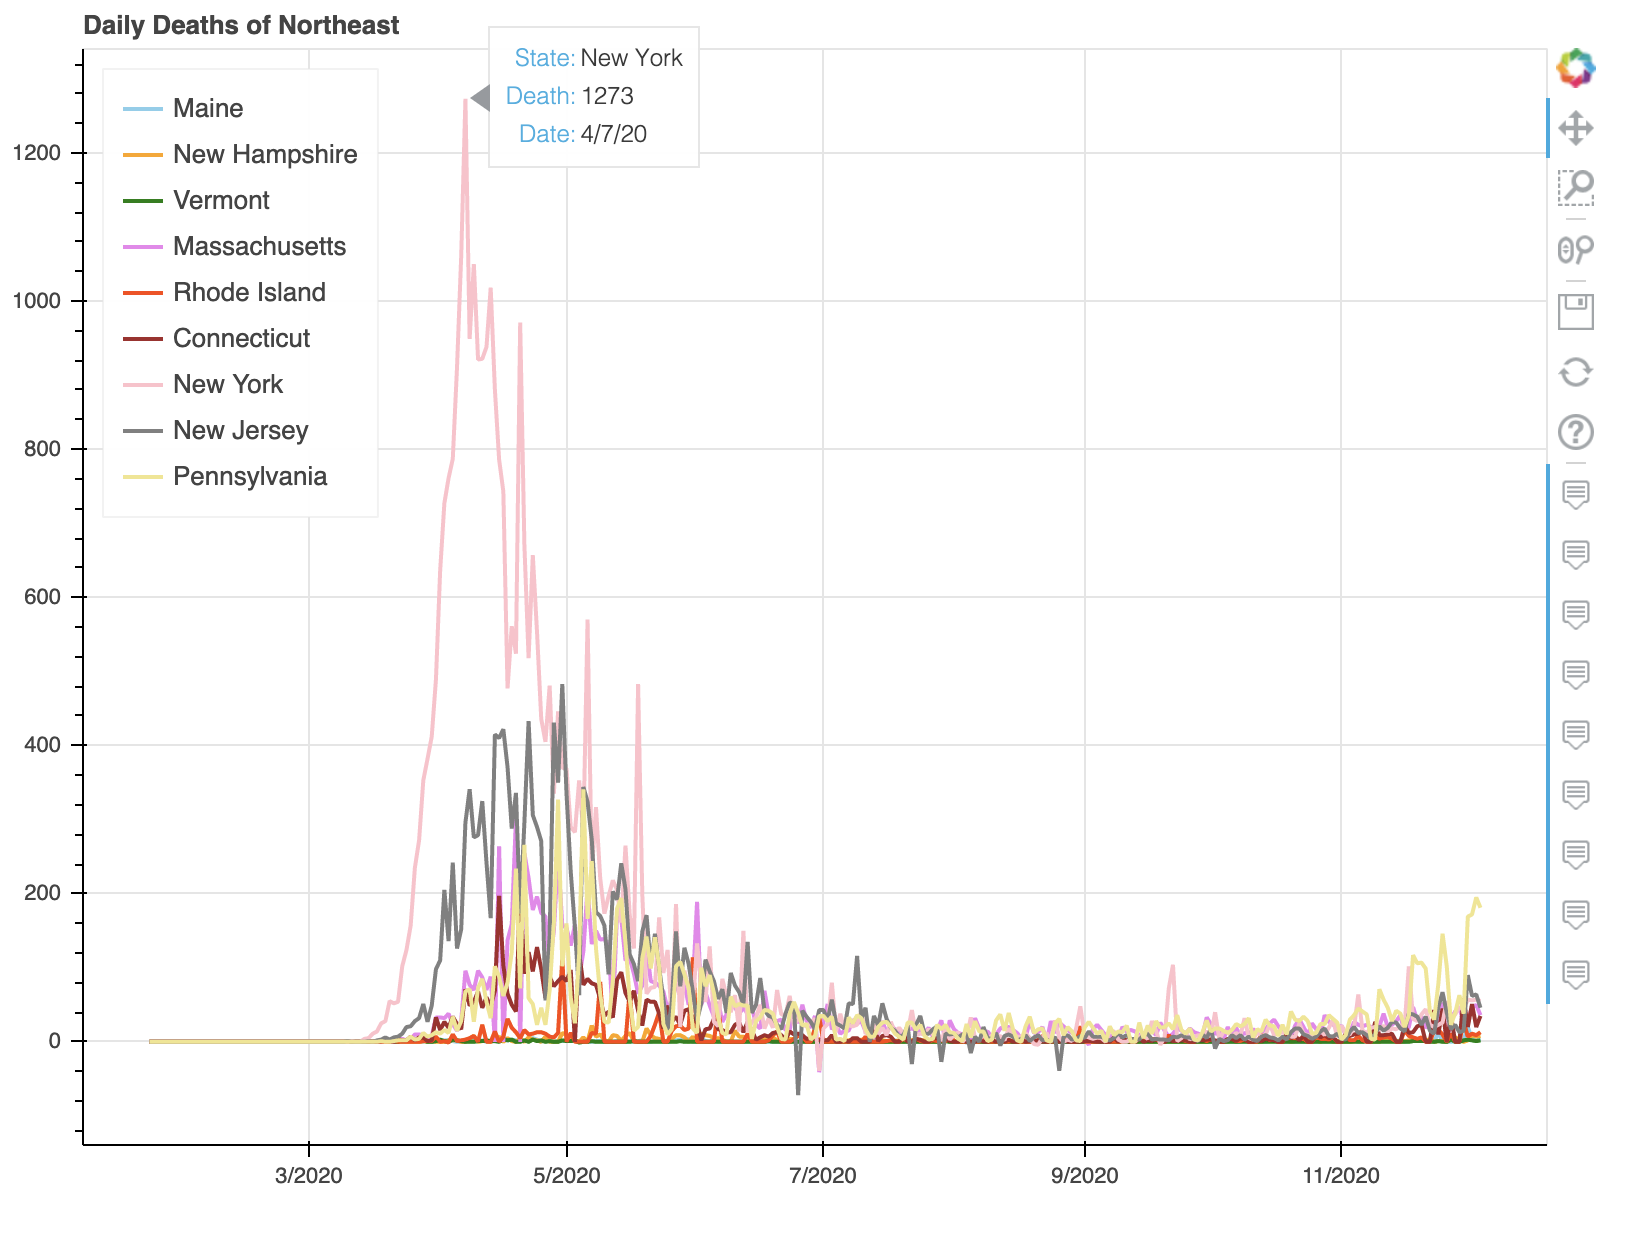
\includegraphics[width=.4\textwidth]{dth_northeast.png}
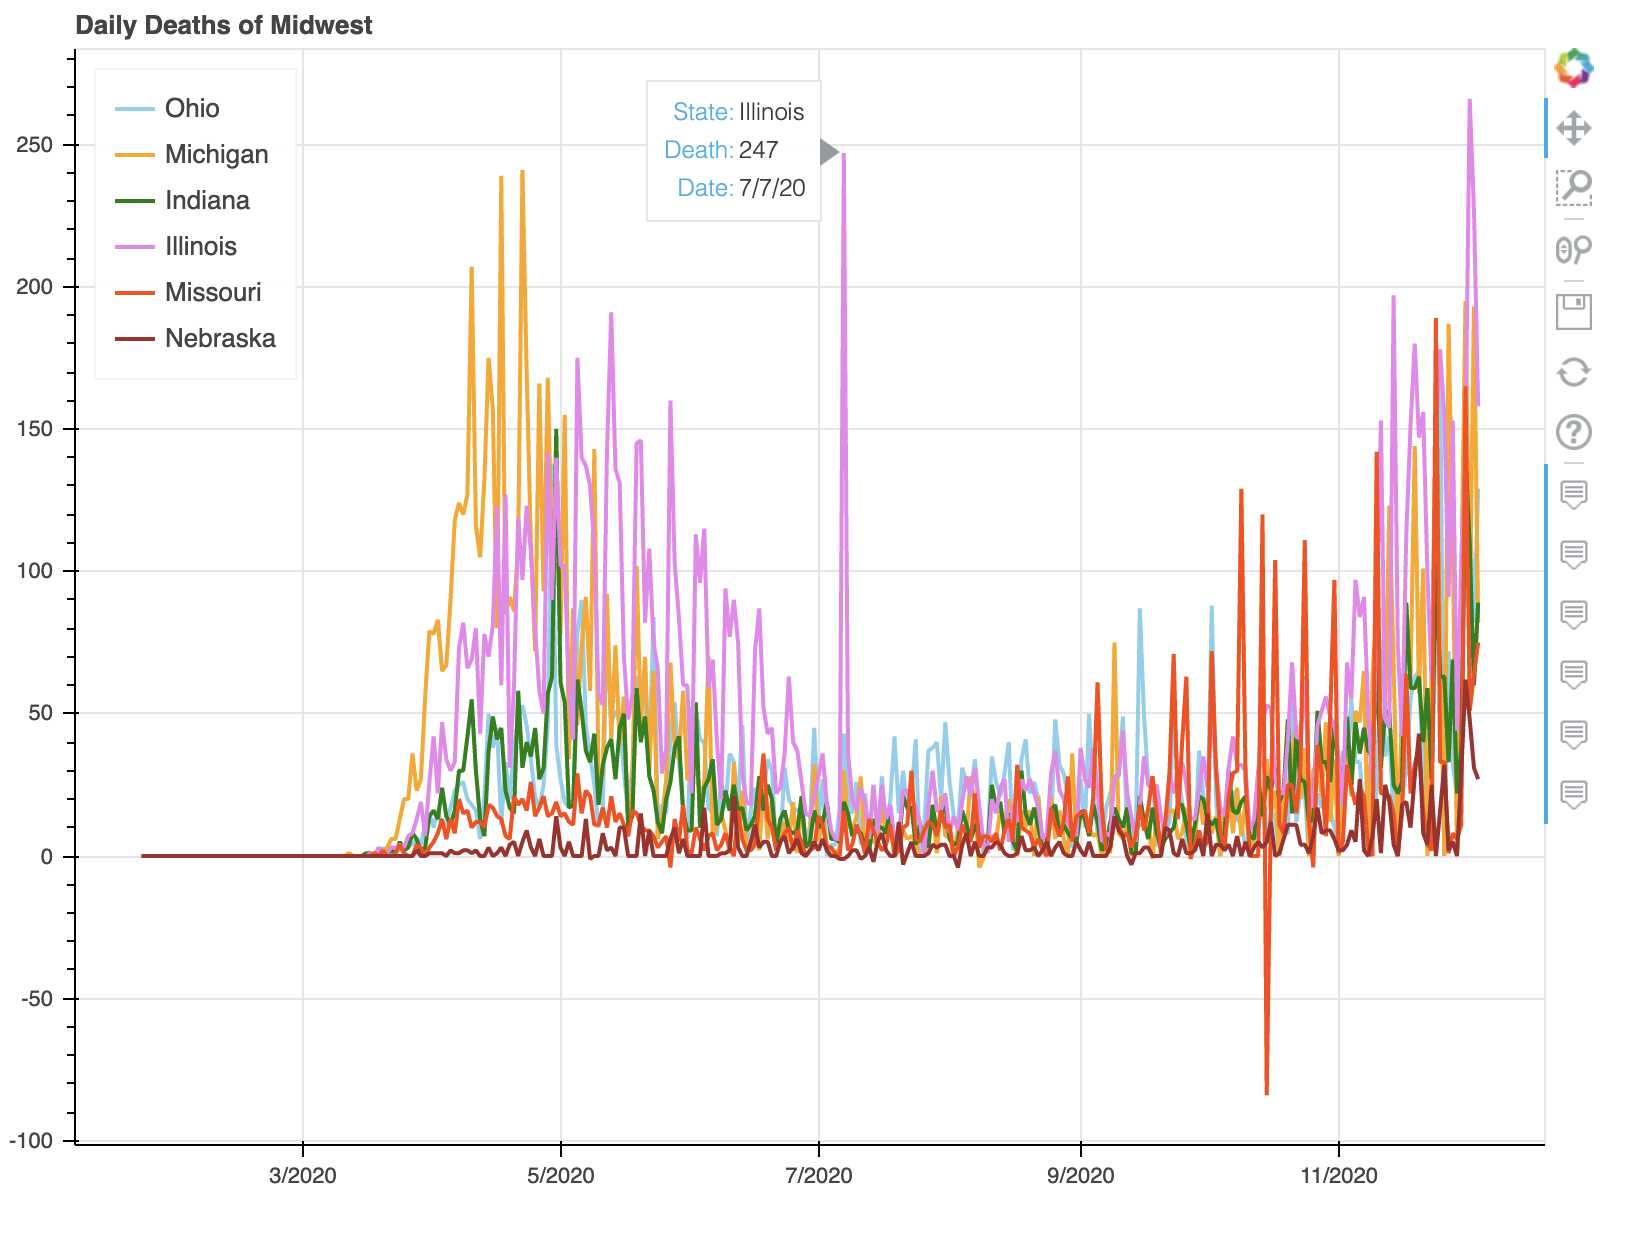
\includegraphics[width=.4\textwidth]{dth_midwest.png}
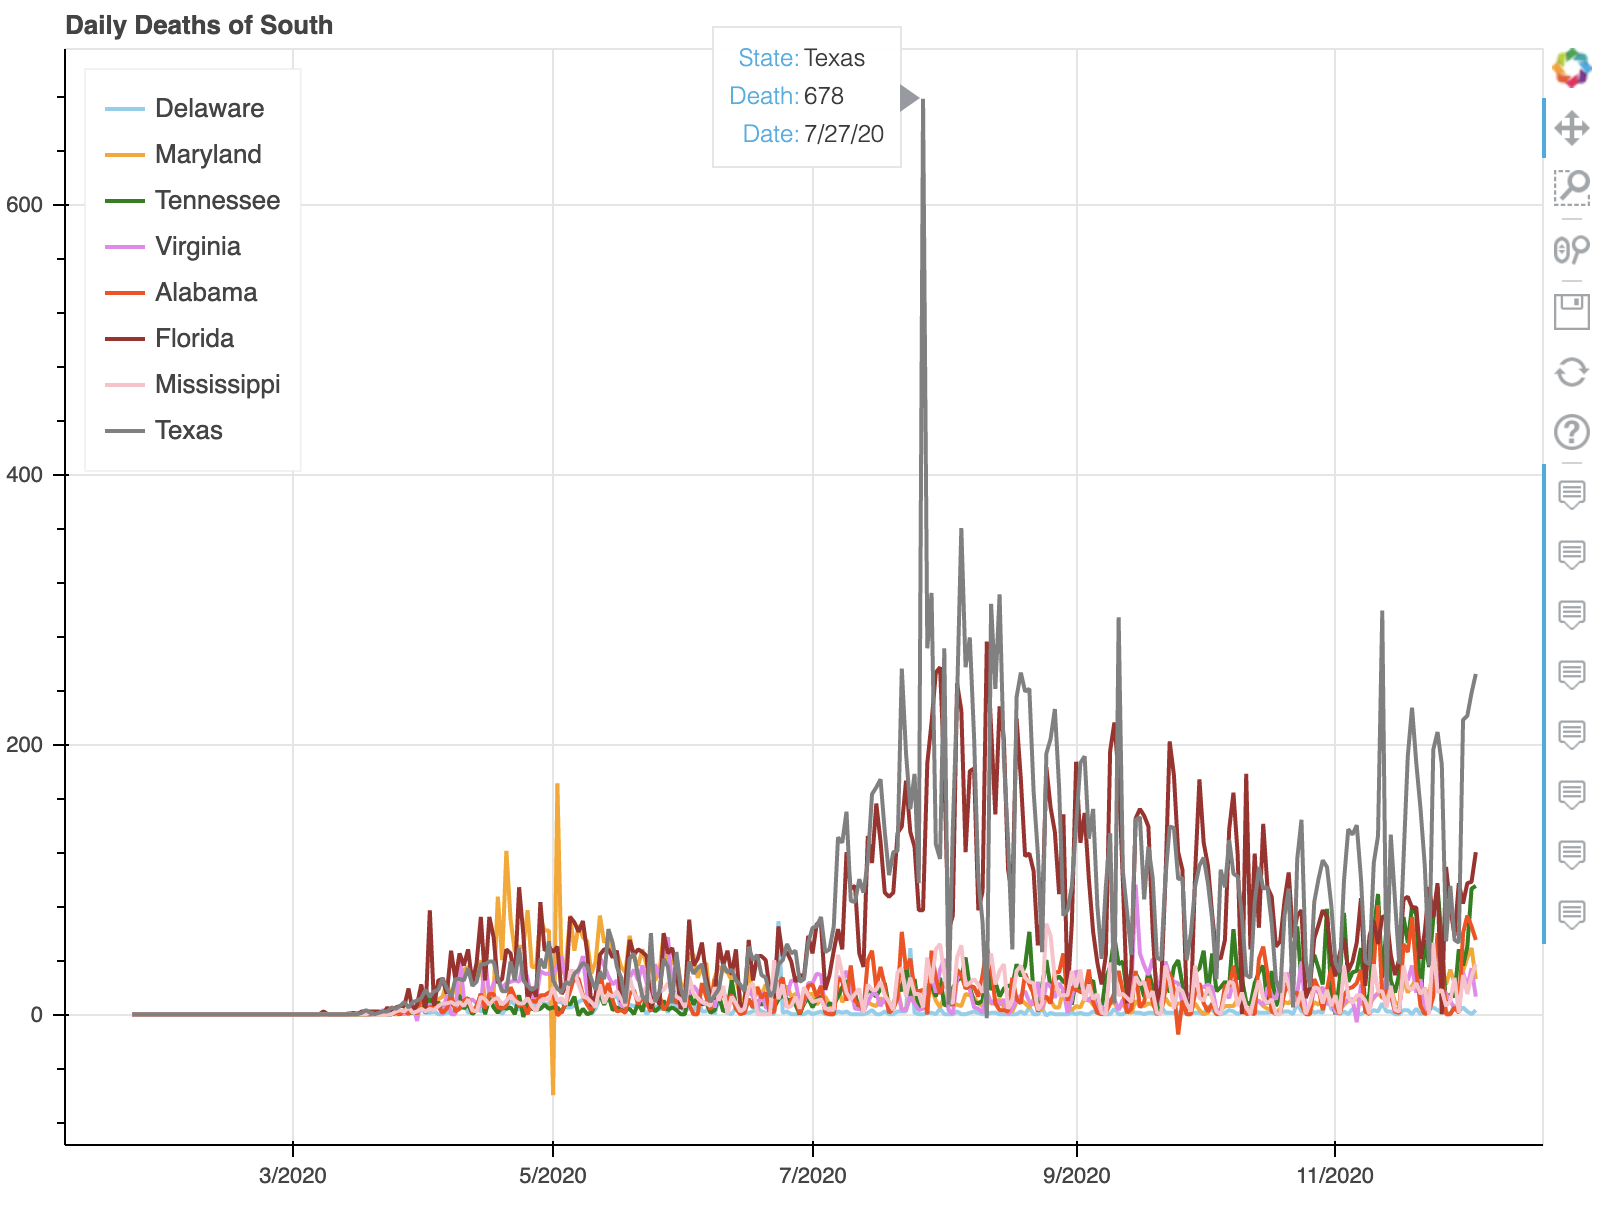
\includegraphics[width=.4\textwidth]{dth_south.png}
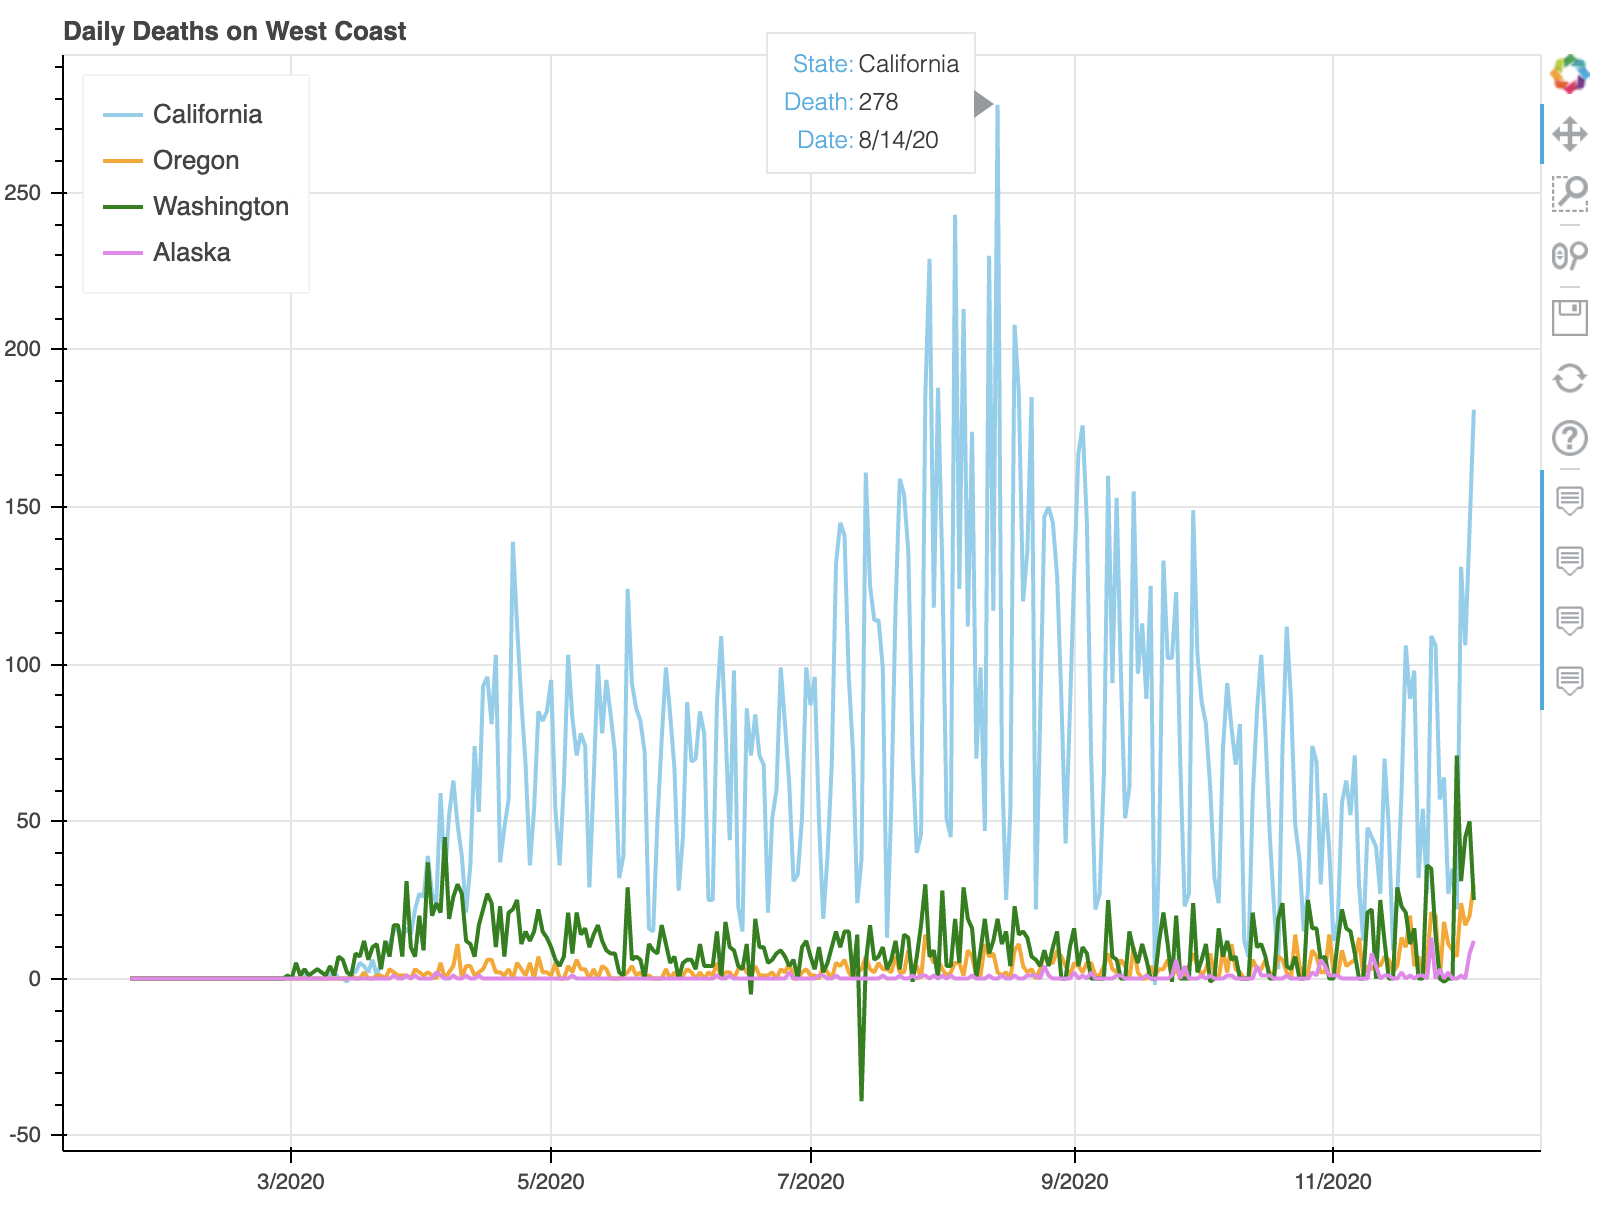
\includegraphics[width=.4\textwidth]{dth_west.png}

\caption{Interactive time series plots of daily deaths of Covid-19 from 1/24/2020 to 12/4/2020 for states in US}
\label{fig:figure}

\end{figure}
\FloatBarrier





It is worth noting that for most of the states in US, the trends of daily deaths are approximately stationary. Therefore, we may plot the sample and the partial autocorrelation function to obtain the orders p and q of ARMA model, and do some time series forecasting. Meanwhile, We observe that several trends contain negative values. This might be due to typos in certain entries. Therefore, some limitations include that there is no data set of recovered cases under the same repository and some entries of current data set seems to be wrong. We may find such data set and correct the negative values of deaths in the future.










\subsection{Interactive Map}


\subsubsection{Implementation}

We aimed to plot an interactive map of US to better visualize the density of cumulative confirmed cases in each state. Specifically, we used the data set of 12/04/2020 which includes confirmed cases, recovered cases, and deaths. By compiling the shape file of US with the Covid-19 data set, we produced the choropleth and filled in color palette based on the confirmed cases, and also added the hover tooltips with information of confirmed, recovered and death cases, using the `bokeh` package.




\subsubsection{Results and Discussion}

\begin{figure}[htp]

\centering
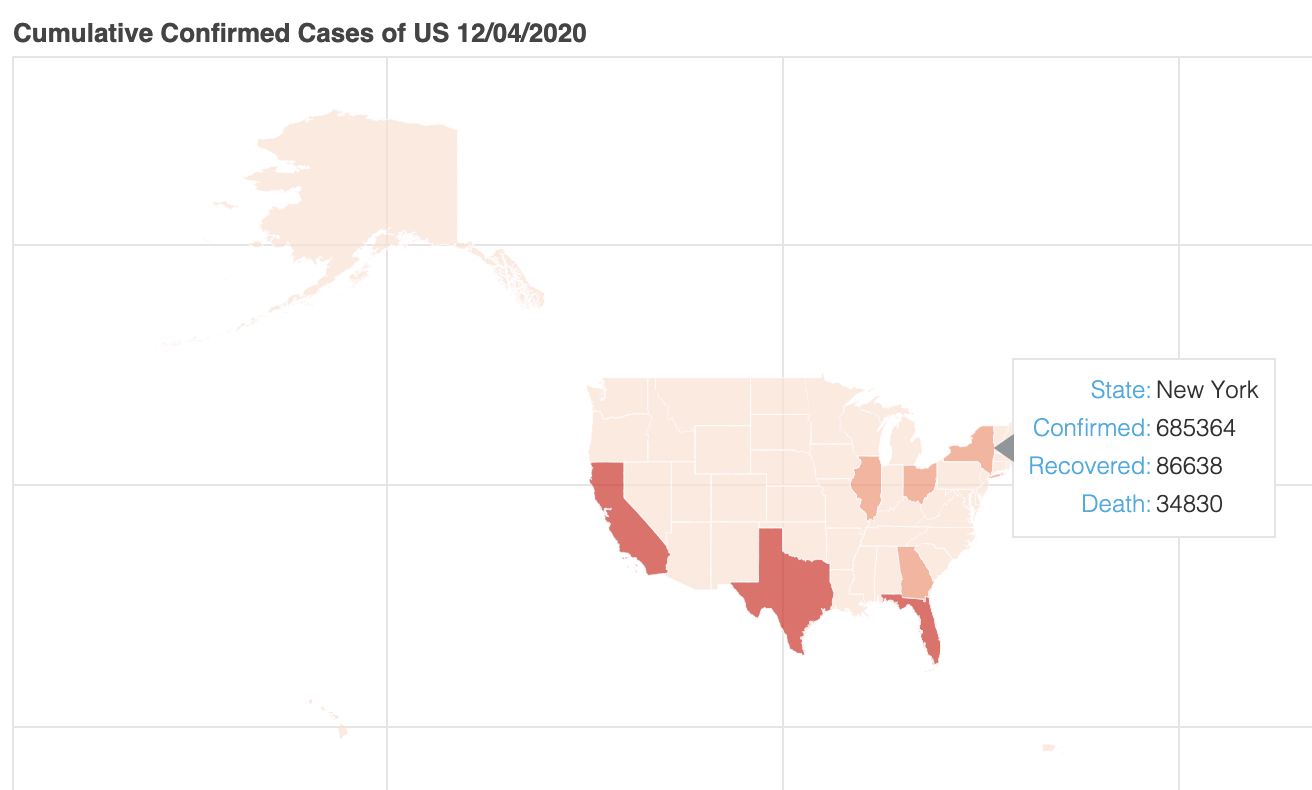
\includegraphics[width=.6\textwidth]{map.png}

\caption{US Choropleth Map for Covid-19 based on cumulative confirmed cases up to 12/04/2020}
\label{fig:figure}
\end{figure}
\FloatBarrier

\noindent
Figure 11 shows that California, Texas, and Florida are the three states under the worst situation. Up to December 4, California has 1310307 confirmed cases in total, while Texas has 1299469 and Florida has 1039207. The states of the second worst group include Illinois with 77088 confirmed cases, New York with 685364, Georgia 496354, and Ohio with 456963. The spread of Covid-19 in the states with large population leads to terrible consequences with great amount of infected individuals and deaths. Therefore, the most efficient way is quarantine, which helps prevent spread of disease, since infected people might unknowingly transmit Covid-19 to others.


In addition, if we have more time, we can produce the choropleth map of deaths and recovered cases to find more interesting things. The limitation is that some states, such as California and Illinois, contain missing values of the recovered population. There might be problem of collecting the recovered data due to large population, but it will be better for future analysis if we can find out the missing values.


As the weather has turned cold, the United States is experiencing the second waves of Covid-19. To enable the world to transition toward normalcy, we should follow the Executive Order and reduce unnecessary outdoor activities, and wear a mask in public places, and take quarantine if necessary.





\section{Bibliography}
The paper that we need to replicate for mask usage \cite{Steff2020mask},  the covid-19 dataset for plotting and simulation \cite{Johnhopkins}, the default value for fitting the covid-19 dataset \cite{Cooper2020SIR}.


\printbibliography






\section{Appendix}

Since we cannot embed the interactive plots in latex and pdf file, we just produce the html files of all plots and put them in the scripts folder.\\

\noindent
Below HTML's are the interactive time series plots of daily confirmed cases of Covid-19 in US.\\

Northeast: DailyNorthEast.html\\

Midwest: DailyMidwest.html\\

South: DailySouth.html\\

West: DailyWestCoast.html\\



\noindent
Below HTML's are the interactive time series plots of daily deaths of Covid-19 in US. \\

Northeast: DeathNorthEast.html\\

Midwest: DeathMidwest.html\\

South: DeathSouth.html\\

West: DeathWestCoast.html\\




\noindent
The HTML for the interactive choropleth map is 12-04-USA.html and is also located in the scripts folder. \\






\end{document}
